\addtocontents{toc}{\protect\newpage}
\chapter{Geometrie von Flächen}

Ziel dieses Kapitels ist es, auf zweidimensionalen Mannigfaltigkeiten (beziehungsweise Flächen im \( \R^3 \)) ``Geometrie'' zu betreiben  (also beispielsweise Längen und Winkel messen und so weiter).\footnote{Für mehr Informationen: \textbf{Gauß} (1827) vgl. \textbf{Spirak}: \emph{A comprehensive introduction to differential geometry} Vol. III --- how to read Gauß}

\section{Reguläre Flächen in \( \R^3 \)}

\begin{remark}[Erinnerung an reguläre Flächen]
  Eine Teilmenge \( S \subset \R^3 \) ist eine \term{reguläre Fläche}, falls es zu jedem Punkt \( p \in S \) eine offene Umgebung \( V \) von \( p \) in \( \R^3 \), eine offene Teilmenge \( U \subset \R^2 \) und eine \( C^\infty \)-Abbildung
  \begin{equation*}
    x: U \ni (u,v) \mapsto x(u,v) = \left( x_1(u,v),x_2(u,v),x_3(u,v) \right) \in \R^3
  \end{equation*}
  gibt mit:
  \begin{enumerate}
    \item \( x(U) = S \cap V \) und \( x: U \to S \cap V \) ist ein Homöomorphismus. 
    \item Das Differenzial \( \text{d}x|_{(u,v)}: \underset{\cong \R^2}{T_{(u,v)}\R^2} \to \underset{\cong \R^3}{T_{x(u,v)}\R^3} \) ist injektiv (\( \forall (u,v) \in U \))
    \begin{itemize}
      \item[\( \Leftrightarrow \)] Die Funktionalmatrix
        \begin{equation*}
          \begin{pmatrix}
            \frac{\partial x_1}{\partial u}(u,v) & \frac{\partial x_1}{\partial v}(u,v) \\
            \frac{\partial x_2}{\partial u}(u,v) & \frac{\partial x_2}{\partial v}(u,v) \\
            \frac{\partial x_3}{\partial u}(u,v) & \frac{\partial x_3}{\partial v}(u,v)
          \end{pmatrix} \eqqcolon \begin{pmatrix}
            x_u(u,v) & x_v(u,v)
          \end{pmatrix}
        \end{equation*}
        hat Rang \( 2 \) (\( \forall (u,v) \in U \)).
      \item[\( \Leftrightarrow \)] \( x_u(u,v) \), \( x_v(u,v) \) sind linear unabhängig (\( \forall (u,v) \in U \)).
      \item[\( \Leftrightarrow \)] Vektorprodukt \( x_u(u,v) \times x_v(u,v) \neq 0 \) (\( \forall (u,v) \in U \)).
    \end{itemize}
  \end{enumerate}
\end{remark}

\begin{figure}[H]
  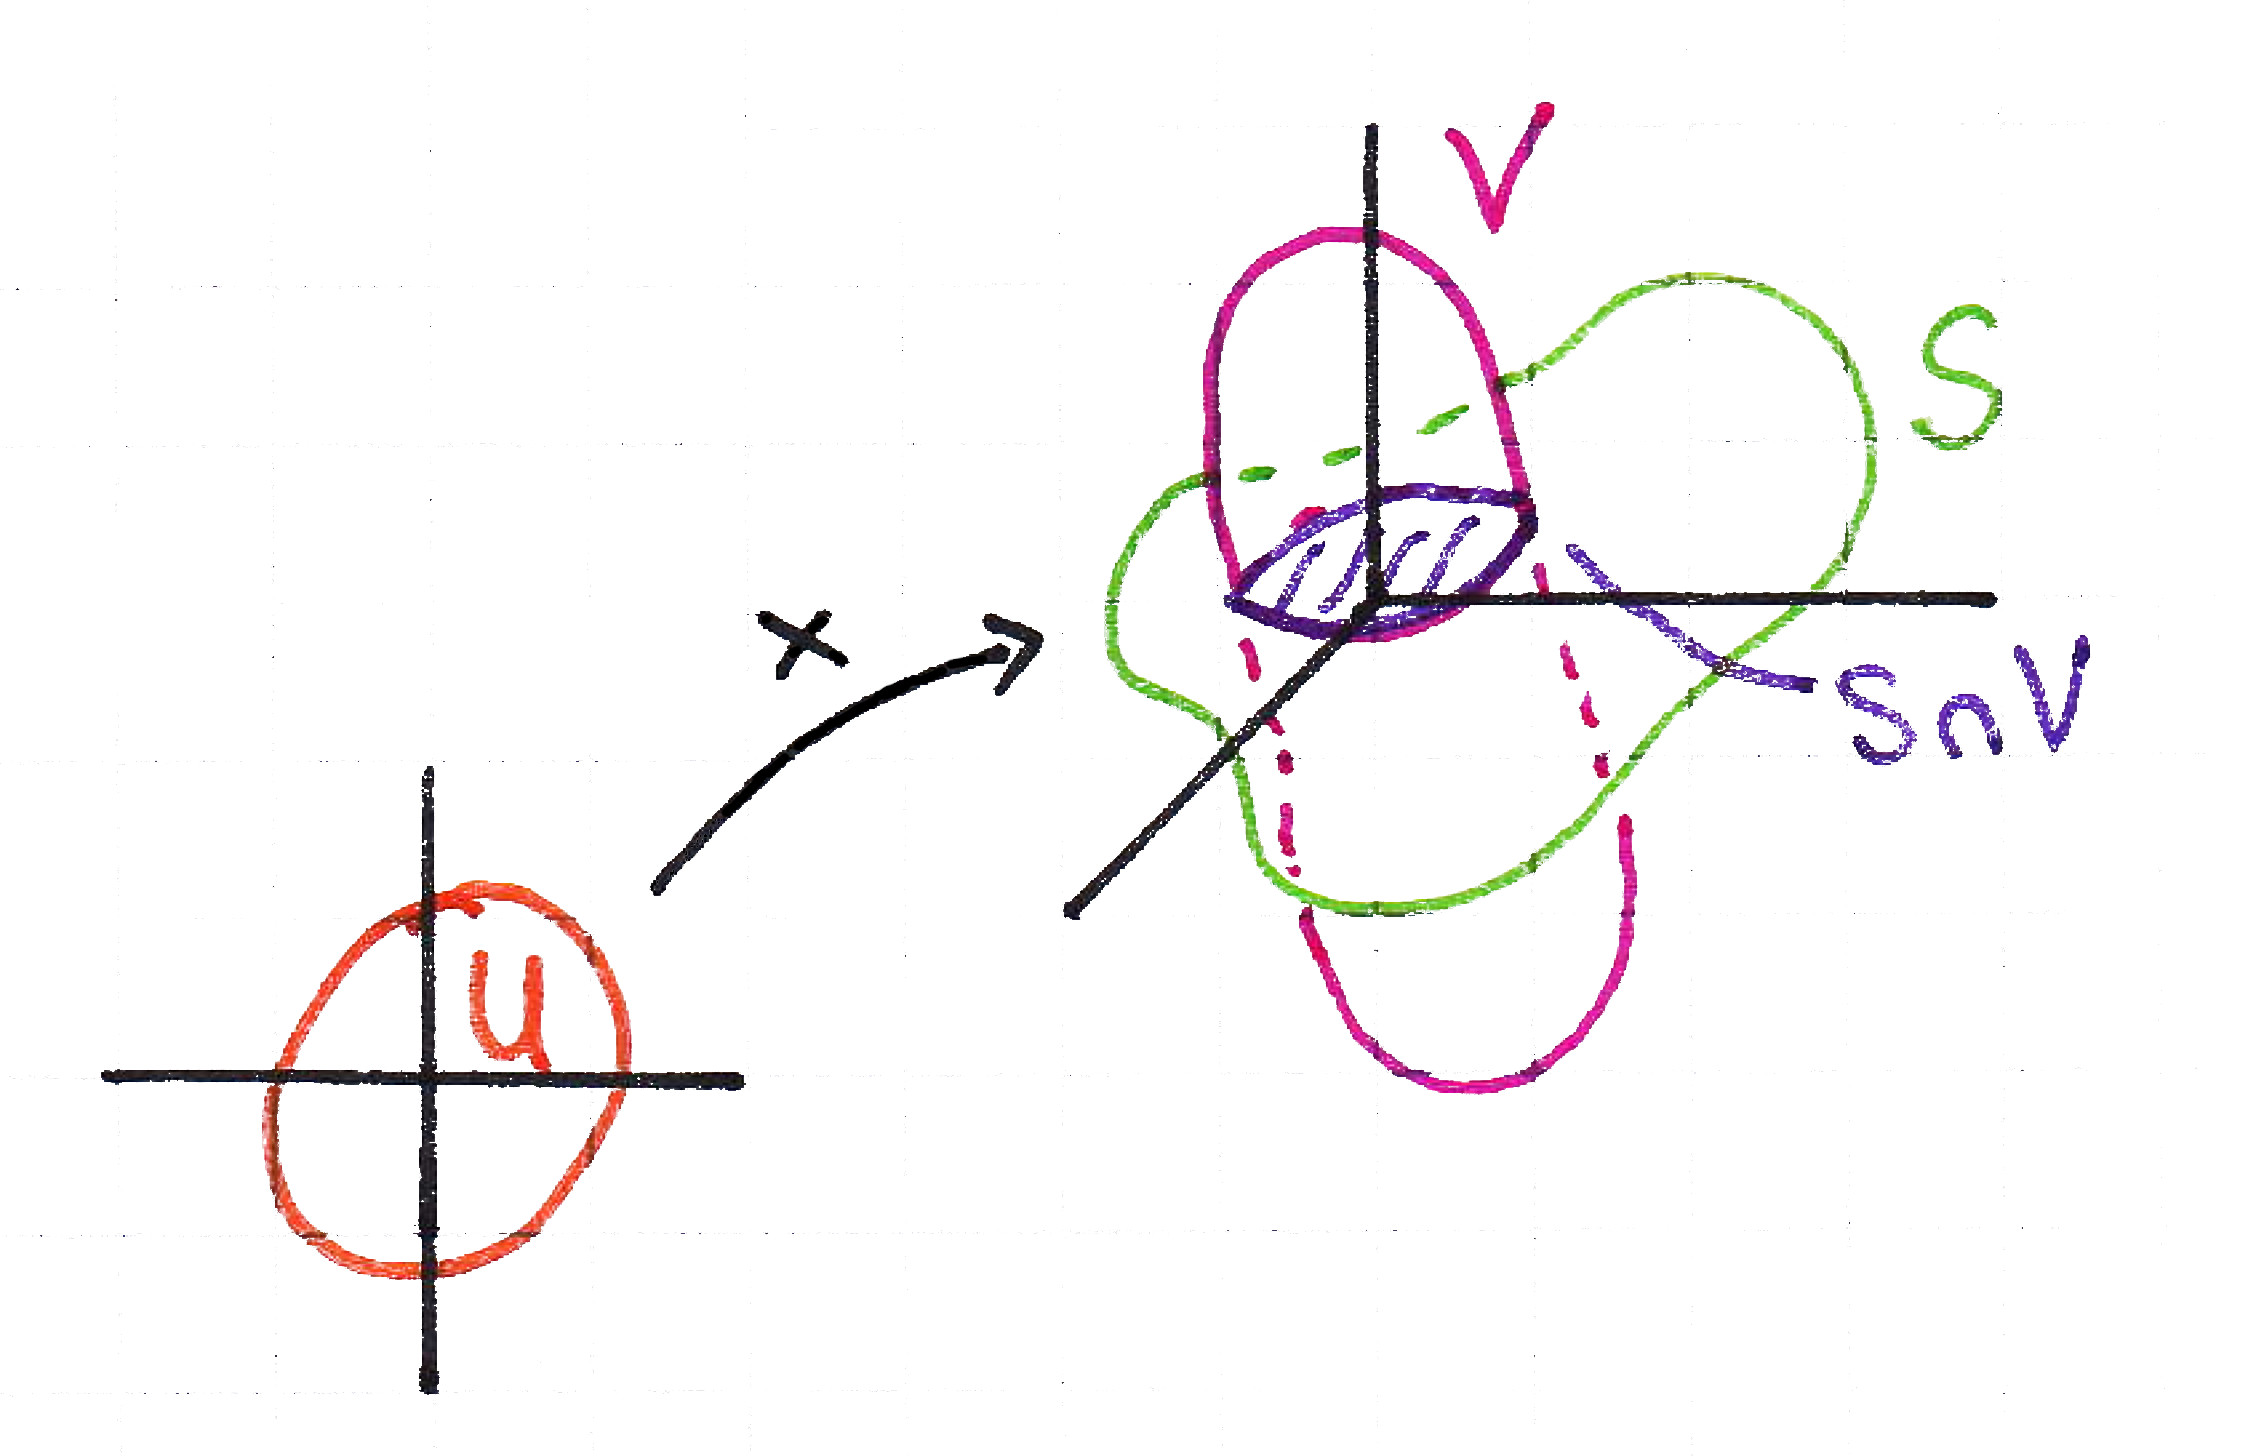
\includegraphics[width=0.6\textwidth]{KonstruktionRegulaereFlaeche}
  \caption{Konstruktion einer regulären Fläche}
\end{figure}

\begin{remark}[Erinnerung an das Kreuz-/Vektorprodukt]
  \  \\
  \( a \coloneqq (a_1, a_2, a_3) \in \R^3 \) und \( b \coloneqq (b_1, b_2, b_3) \in \R^3 \).
  \begin{equation*}
    a \wedge b \ (\cong a \times b) \ \coloneqq (a_2b_3-a_3b_2, a_3b_1-a_1b_3, a_1b_2-a_2b_1) \in \R^3\text{.}
  \end{equation*}
  \emph{Eigenschaften}:
  \begin{enumerate}
    \item \( a \wedge b \bot a \) \quad \( a \wedge b \bot b \)
    \item \( \det(a, b, a \wedge b) \geq 0 \)
    \item \( a \wedge (-b) = - (a \wedge b) \)
    \item \( \Vert a \wedge b \Vert = \Vert a \Vert * \Vert b \Vert * \sin \alpha \) (Winkel zwischen den Vektoren), Fläche des von \( a \) und \( b \) aufgespannten Parallelogramms
  \end{enumerate}
\end{remark}

\begin{definition}[Tangentialraum]
  Der \term{Tangentialraum}\label{def:tangentialraum} in Punkt \( p \in \R^3 \) ist der affine Unterraum
  \begin{equation*}
    T_p\R^3 \coloneqq \{ p \} \times \R^3 = \{ (p,v) : v \in \R^3 \}\text{.}
  \end{equation*}
  Für eine reguläre Fläche \( S \) und \( p = x(u,v) \in S \) ist die \term{Tangentialebene}\label{def:tangentialebene} in \( p \in S \) definiert als
  \begin{equation*}
    T_p S \coloneqq \text{d}x_{(u,v)}\left(T_{(u,v)}\R^2\right) \coloneqq \{ p \} \times [x_u(u,v), x_v(u,v)] \subset T_p\R^3
  \end{equation*}
  \( 2 \)-dimensionaler, affiner Unterraum des \( \R^3 \).
\end{definition}

\begin{remark}[Geometrische Interpretation des Tangentialraums]
  \
  \begin{equation*}
    x_u(u_0,v_0) = \frac{\partial x}{\partial u}(u_0,v_0) = \frac{\text{d}}{\text{d}t}|_{t = 0}x(u_0+t,v_0) = \text{d}x|_{(u_0,v_0)}(e_1)
  \end{equation*}
  \emph{Allgemein}: \\*
  Sei \( c(t) \coloneqq x(u(t),v(t)) \) eine \term{Flächenkurve}\label{def:flaechenkurve} in \( x(U) \) durch den Punkt \( x(u(0),v(0)) = x(u_0,v_0) \). \\*
  \term{Tangentialvektor}\label{def:tangentialvektor} an \( c \) im Punkt \( x(u_0,v_0) \):
  \begin{align*}
    c'(0) &= \frac{\text{d}c}{\text{d}t}|_{t=0} = \frac{\text{d}}{\text{d}t}x(u(t),v(t))|_{t = 0}\\
    &= \frac{\partial x}{\partial u}(u(0),v(0))\,u'(0) + \frac{\partial x}{\partial v}(u(0),v(0))\,v'(0) = x_u(u_0,v_0)u'(0)+x_v(u_0,v_0)v'(0)
  \end{align*}
  \emph{Also}: Tangentialebene in \( x(u_0,v_0) = \) Menge aller Tangentialvektoren als Flächenkurven.
\end{remark}

\begin{figure}[H]
  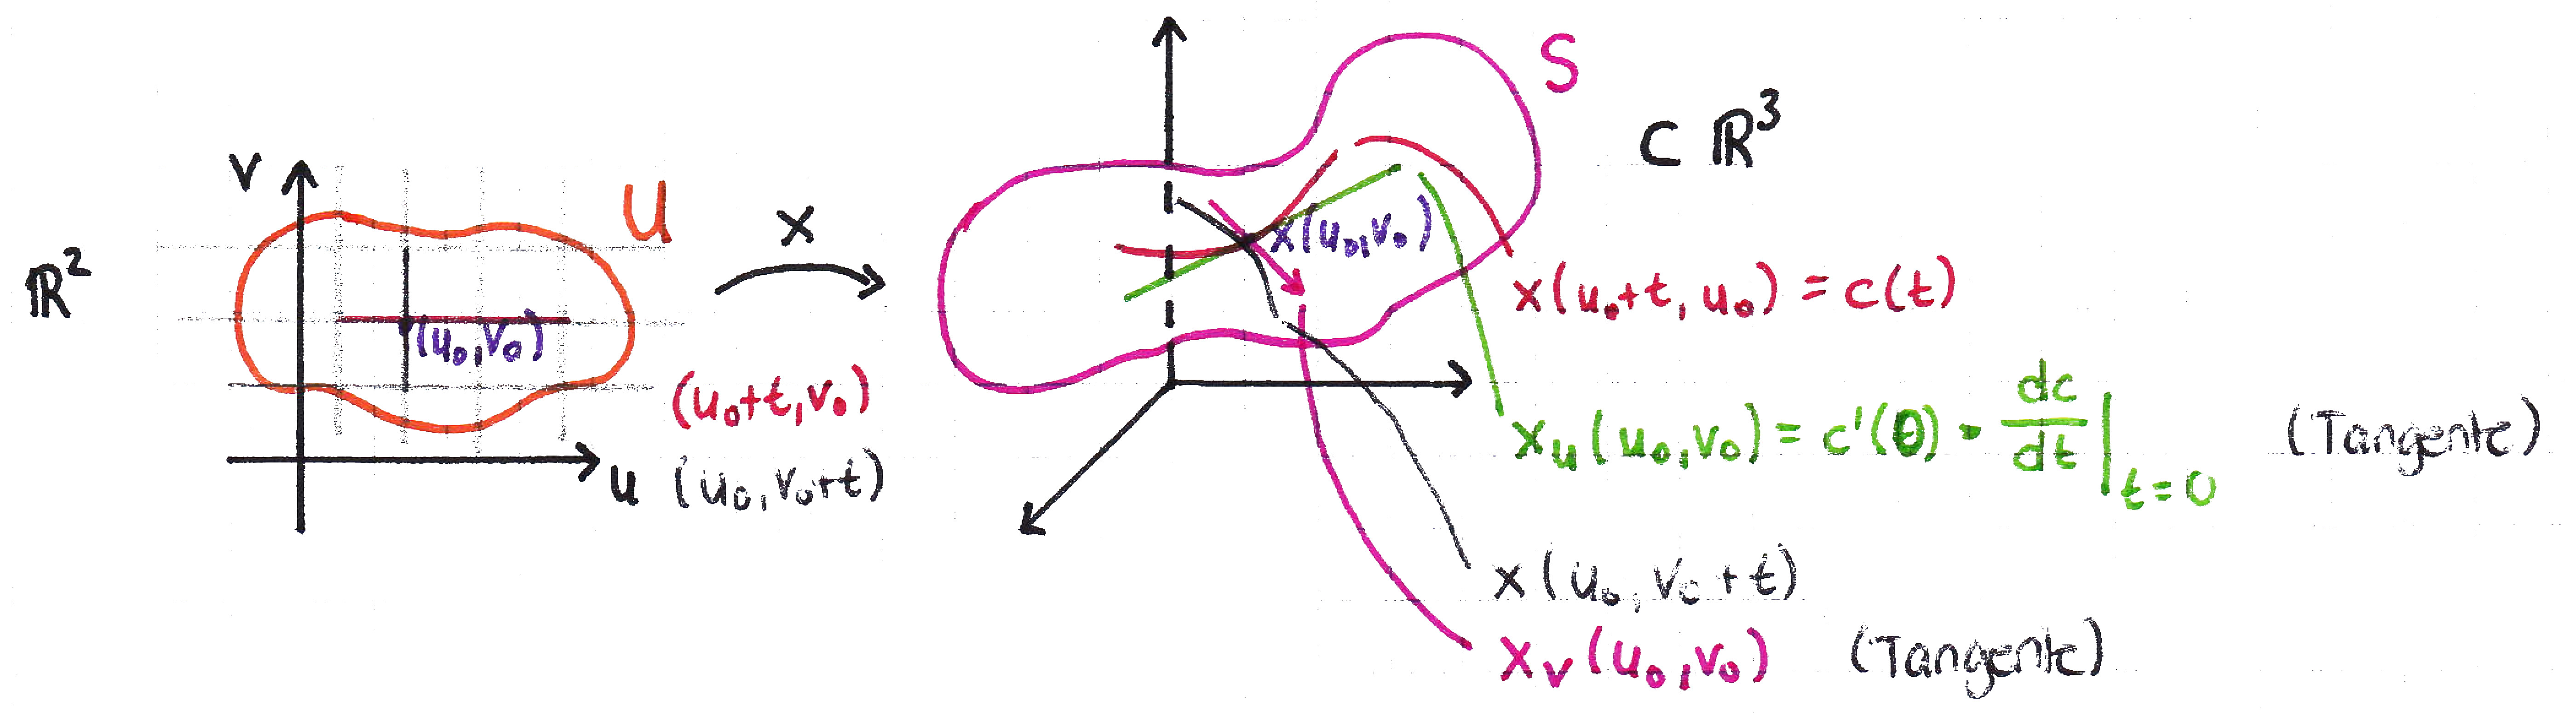
\includegraphics[width=\textwidth]{TangentialraumGeometrisch}
  \caption{Geometrische Interpretation des Tangentialraums}
\end{figure}

\begin{remark}[Parameterisierungsunabhängigkeit obiger Definitionen]
  \  \\
  Sei \( \overline{x} : \overline{U} \to \overline{x}(\overline{U}) = x(U) \) eine andere Parametrisierung von \( S \) um \( p = x(u_0, v_0) = \overline{x}(\overline{u_0}, \overline{v_0}) \). \\
  \emph{Zu zeigen}: Die lineare Hüllen sind gleich: \( [\overline{x}_{\overline{u}}, \overline{x}_{\overline{v}}] = [x_u, x_v] \). \\
  Es ist \( k \coloneqq \overline{x}^{-1}*x : U \to \overline{U} \) die Koordinatentransformation:
  \begin{equation*}
    x_u = \frac{\partial x}{\partial u}(u,v) = \frac{\partial \overline{x}(\overline{x}^{-1} \circ x)}{\partial u}(u,v) = \frac{\partial \overline{x}}{\partial u}(\overline{u}, \overline{v}) = \frac{\partial \overline{x}}{\partial \overline{u}}(\overline{u},\overline{v}) *\frac{\partial \overline{u}}{\partial u}(u,v)+\frac{\partial \overline{x}}{\partial \overline{v}} * \frac{\partial \overline{v}}{\partial u}
  \end{equation*}
  Entsprechend:
  \begin{align*}
    x_u &= \overline{x}_{\overline{u}}\frac{\partial \overline{u}}{\partial u} + \overline{x}_{\overline{v}}\frac{\partial \overline{v}}{\partial u} \quad \text{d.h. \( x_u \) ist Linearkombination von \( \overline{x}_{\overline{u}} \) und \( \overline{x}_{\overline{v}} \)} \\
    x_v &= \overline{x}_{\overline{u}}\frac{\partial \overline{u}}{\partial v} + \overline{x}_{\overline{v}}\frac{\partial \overline{v}}{\partial v} \quad \text{d.h. \( x_v \) ist Linearkombination von \( \overline{x}_{\overline{u}} \) und \( \overline{x}_{\overline{v}} \)}
  \end{align*}
  Also \( [x_u, x_v] = [\overline{x}_{\overline{u}}, \overline{x}_{\overline{v}}] \), verschiedene Basen von \( T_p S \) mit Basis-Transformations-Matrix
  \begin{equation*}
    D(u,v) = \begin{pmatrix}
      \frac{\partial \overline{u}}{\partial u} & \frac{\partial \overline{u}}{\partial v} \\
      \frac{\partial \overline{v}}{\partial u} & \frac{\partial \overline{v}}{\partial v}
    \end{pmatrix}\text{.}
  \end{equation*}
  Das ist die Funktionalmatrix der Parametertransformation. Insbesondere ist \( \det D(u,v) \neq 0 \).
\end{remark}

\begin{figure}[H]
  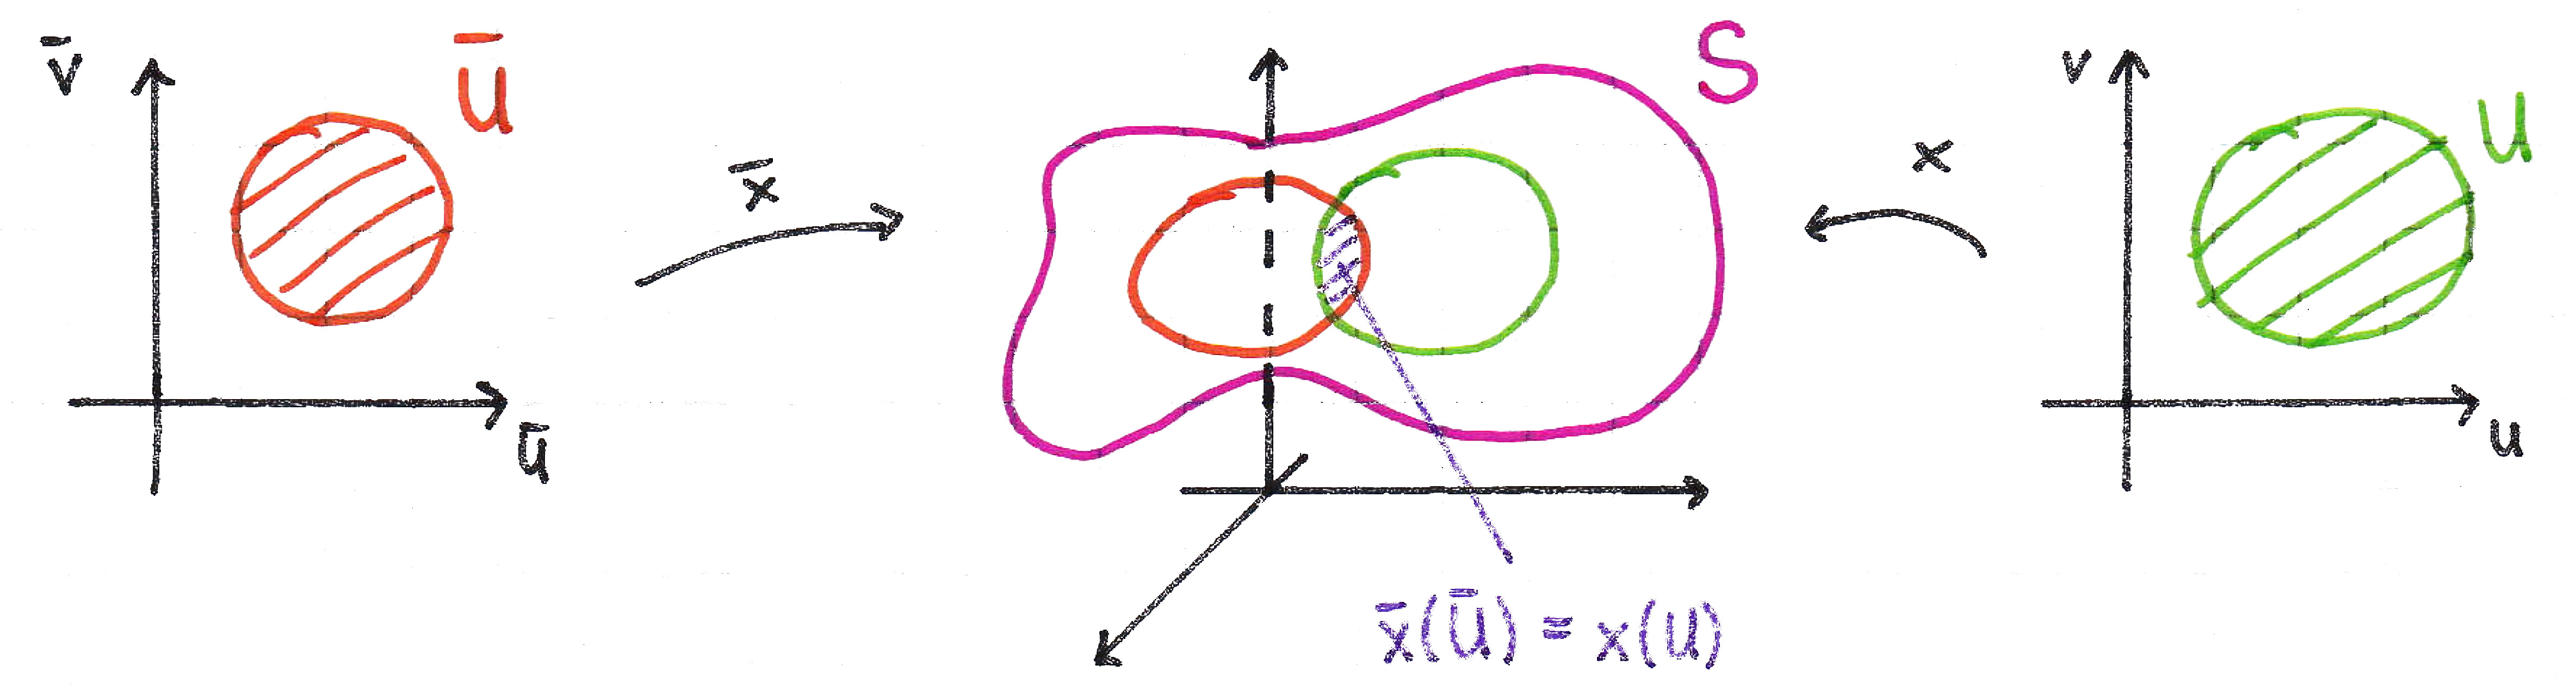
\includegraphics[width=.8\textwidth]{ParametrisierungTangentialraum}
  \caption{Parameterisierungsunabhängigkeit der Definition des Tangentialraums}
\end{figure}

\begin{example}
  \
  \begin{enumerate}
    \item \emph{affine Ebene}: \( a_0, a, b \in \R^3 \), \( S \coloneqq \{ a_0 + ua + vb : u,v \in \R \} \) ist reguläre Fläche, falls \( a \) und \( b \) linear unabhängig sind. Mit
    \begin{equation*}
      U \coloneqq \R^2, \ V \coloneqq \R^3, \ x: \R^2 \ni (u,v) \mapsto a_0 + ua + vb \in \R^3\text{,}
    \end{equation*}
    \begin{equation*}
      x_u  =\frac{\partial x}{\partial u} = a, \ x_v = \frac{\partial x}{\partial v} = b, \ T_{x(u,v)}S = \{ x(u,v) \} \times [a,b] \cong S\text{.}
    \end{equation*}

    \item \( U \subseteq \R^2 \), \( f: U \to \R \) \( C^\infty \)-Funktion, \( S \coloneqq \) Graph von \( f \coloneqq \{ (x_1, x_2, x_3) \in \R^3 : (x_1, x_2) \in U, \ x_3 = f(x_1, x_2) \} \). \\
    \emph{Behauptung}: \( S \) ist reguläre Fläche. \\
    \( U = U \), \( V = \R^3 \), \( x : U \ni (u,v) \mapsto (u,v, f(u,v)) \in \R^3 \). \\
    \( x(U) = S = S \cap V \), \( x: U \to S \) stetig und \( x^{-1}: S \ni (u,v,f(u,v)) \mapsto (u,v) \in U \) ist als Projektion auch stetig. Also ist \( x \) ein Homöomorphismus. \\
    Weiter ist
    \begin{align*}
      x_u &= \left(1,0, \frac{\partial f}{\partial u}\right), \\
      x_v &= \left( 0,1, \frac{\partial f}{\partial v} \right)
    \end{align*}
    also sind \( x_u \) und \( x_v \) linear unabhängig.
  \end{enumerate}
\end{example}

\begin{remark}
  Ist \( S \) reguläre Fläche in \( \R^3 \), so existiert zu jedem Punkt \( p \in S \) eine offene Umgebung \( O \subset \R^3 \), so dass \( S \cap O \) Graph einer \( C^\infty \)-Funktion ist (beispielsweise \( S^2 = \) 2-Sphäre vom Radius \( 1 \)).
\end{remark}

\section{Erste Fundamentalform einer regulären Fläche}

\begin{remark}[Erinnerung an LA]
  Modell der euklidischen Geometrie: \\*
  \( \R \)-Vektorraum + Skalarprodukt = euklidischer \( (V, \langle \cdot, \cdot \rangle) \)-Vektorraum \\*
  \( \leadsto \Vert a \Vert = \sqrt{\langle a, a \rangle} \) \textbf{Länge} eines Vektors \( a \in V \) \\*
  \( \leadsto \cos \measuredangle(a,b) = \frac{\langle a, b \rangle}{\Vert a \Vert*\Vert b \Vert} = \left\langle \frac{a}{\Vert a \Vert}, \frac{b}{\Vert b \Vert} \right\rangle \) \textbf{Winkel} \\
\end{remark}

\begin{remark}[Übertragung auf gekrümmte Flächen (Gauß)]
  Sei \( S \) eine reguläre Fläche und \( p \in S \). Betrachte die bilineare Abbildung
  \begin{equation*}
    \langle \cdot, \cdot \rangle_p : T_p S \times T_p S \to T_p S\text{,} \quad \langle a, b \rangle_p \coloneqq \langle a, b \rangle
  \end{equation*}
  (identifiziere affine Ebene mit VR \( R^2 \), \( \langle a, b \rangle \) ist Standard-SKP in \( \R^3 \)). \\
  Die Zuordnung \( I: p \mapsto I_p \coloneqq \langle \cdot, \cdot \rangle_p \) heißt \term{Erste Fundamentalform der Fläche \( S \)}\label{def:ersteFundamentalform}. \\
  Ist \( x: U \ni (u,v) \mapsto x(u,v) \in S \) eine lokale Parametrisierung von \( S \) (um \( p \in S \)), so bilden \( x_u(u,v) \) und \( x_v(u,v) \) eine Basis von \( T_{x(u,v)}S \). Bezüglich dieser können wir \( I_p \), \( p \in x(U) \subset S \) durch eine positiv definite symmetrische \( 2 \times 2 \)-Matrix darstellen:
  \begin{equation*}
      \left( \underbrace{g_{ij}(u,v)}_{\in \R^{2 \times 2}} \right) = \begin{pmatrix}
        g_{11}(u,v) & g_{12}(u,v) \\
        g_{21}(u,v) & g_{22}(u,v)
      \end{pmatrix} = \underset{\text{Originalnotation Gauß}}{\begin{pmatrix}
        E(u,v) & F(u,v) \\
        F(u,v) & G(u,v)
      \end{pmatrix}}
  \end{equation*}
  mit
  \begin{align*}
    g_{11}(u,v) = E(u,v) &= \langle x_u(u,v),x_u(u,v) \rangle_p = \underset{\text{Standard-SKP von }\R^3}{\langle x_u(u,v),x_u(u,v) \rangle} \\
    g_{12}(u,v) &= \langle x_u, x_v \rangle_p = \langle x_v, x_u \rangle = g_{21}(u,v) \\
    g_{22}(u,v) &= \langle x_v, x_v \rangle_p = \langle x_v, x_v \rangle
  \end{align*}
  insbesondere sind die \( g_{ij}: U \to \R \) \( C^\infty \)-Funktionen. \\
  \emph{Also}: \( \left( g_{ij}(u,v) \right) \) ist eine Familie \( \in \R^{2\times 2} \) von Skalarprodukten, die differenzierbar von \( (u,v) \) abhängig ist. (Riemannsche Metrik)
\end{remark}

\begin{remark}[Bedingungen an obige Matrix]
  \
  \begin{enumerate}
    \item \emph{Hurwitz}: \( I_p \) ist positiv definit \( \Leftrightarrow E = g_{11} > 0 \), \( E*G-F^2 = \det(g_{ij}) > 0 \).
    \item \emph{andere Parametrisierung}: \( \overline{x}(\overline{u},\overline{v}) \leadsto \) neue Basis \( \{ \overline{x}_{\overline{u}}, \overline{x}_{\overline{v}} \} \), Matrix von \( I \) bezüglich dieser Basis \( \left( \underset{\in \R^{2\times 2}}{\overline{g}_{ij}(\overline{u}, \overline{v})} \right) \) mit
    \begin{equation*}
      \left( g_{ij}(u,v) \right) = D{(u,v)}^\top(\overline{g}_{ij}(\overline{u},\overline{v}))D(u,v)
    \end{equation*}
    mit 
    \begin{equation*}
      D(u,v) = \begin{pmatrix}
        \frac{\partial \overline{u}}{\partial u} & \frac{\partial \overline{u}}{\partial v} \\
        \frac{\partial \overline{v}}{\partial u} & \frac{\partial \overline{v}}{\partial v}
      \end{pmatrix}\text{,}
    \end{equation*}
    siehe auch Basiswechselmatrix.
  \end{enumerate}
\end{remark}

\begin{example}[Beispiele zur ersten Fundamentalform]
  \
  \begin{enumerate}

    \item \( S \coloneqq \) affine Ebene \( \subset \R^3 \): \( a \), \( b \): \( \Vert a \Vert = \Vert b \Vert = 1 \), \( \langle a, b \rangle = 0 \) (also \( a \bot b \)) \\
    \emph{Parametrisierung}: \( x(u,v) = a_0 + ua + vb \), \( (u,v) \in \R^2 = U \).
    \begin{align*}
      x_u &= \frac{\partial x}{\partial u} = a, \quad x_v = \frac{\partial x}{\partial v} = b\text{,} \\
      E &= \langle x_u, x_u \rangle = \langle a, a \rangle = \Vert a \Vert^2 = 1 \\
      F &= \langle x_u, x_v \rangle = \langle a, b \rangle = 0 \\
      G &= \langle x_v, x_v \rangle = \langle b, b \rangle = \Vert b \Vert^2 = 1 \\
      &\leadsto \begin{pmatrix}
        E & F \\
        F & G
      \end{pmatrix}(u,v) = \begin{pmatrix}
        1 & 0 \\
        0 & 1
      \end{pmatrix}
    \end{align*}

    \item \( S = \) Zylinder \( = \left \{ (x_1, x_2, x_3) \in \R^3 : x_1^2+x_2^2 = r^2 \right \} \) \\
    \emph{Lokale Parametrisierung} (als Rotationsfläche):
    \begin{equation*}
      x(u,v) = (r \cos u, r \sin u, v), \quad (u,v) \in U = (0,2\pi) \times \R \subset \R^2\text{.}
    \end{equation*}
    \begin{align*}
      x_u &= \frac{\partial x}{\partial u} = r(-\sin u, \cos u, 0)\text{,} \\
      x_v &= \frac{\partial x}{\partial v} = (0,0,1)\text{,} \\
        &\leadsto \begin{pmatrix}
          E & F \\
          F & G
        \end{pmatrix}(u,v) = \begin{pmatrix}
          r^2 & 0 \\
          0 & 1
  	\end{pmatrix} \text{ konstant}
    \end{align*}
    \emph{Bemerkung}: Für \( r = 1 \) ist die erste Fundamentalform des Zylinders identisch mit der ersten Fundamentalform der Ebene. \\
    \emph{Grund}: Ebene und Zylinder sind lokal isometrisch (haben im Kleinen die gleiche Geometrie): auf- und abwickeln. Insbesondere sagt die erste Fundamentalform nichts darüber aus, wie die Fläche in \( \R^3 \) eingebettet ist.

    \item \( S = S_R^2 = \) Sphäre vom Radius \( R \) \\
    \emph{Lokale Parametrisierung} (mit geographischen Koordinaten):
    \begin{align*}
      (\theta, \phi) &\in (-\frac{\pi}{2}, \frac{\pi}{2}) \times (0, 2\pi) = U \\
      x(\theta, \phi) &= \left( R\cos \theta \cos \phi, R \cos \theta \sin \phi, R \sin \theta \right)\text{,} \\
      x_\theta &= \frac{\partial x}{\partial \theta} = \left( - R \sin \theta \cos \phi, -R \sin \theta \sin \phi, R \cos \theta \right)\text{,} \\
      x_\phi &= \frac{\partial x}{\partial \phi} = \left( - R \cos \theta \sin \phi, R \cos \theta \cos \phi, 0 \right)
    \end{align*}
    Erste Fundamentalform: \( I(\theta, \phi) = \begin{pmatrix}
      \langle x_\theta, x_\theta \rangle & \langle x_\theta, x_\phi \rangle \\
      \langle x_\phi, x_\theta \rangle & \langle x_\phi, x_\phi \rangle
    \end{pmatrix} = \begin{pmatrix}
        R^2 & 0 \\
        0 & R^2\cos^2 \theta
      \end{pmatrix} \)
  \end{enumerate}
\end{example}

\begin{remark}[Wozu ist die erste Fundamentalform gut?]
 \
 \begin{enumerate}

   \item \emph{Längen}: Mithilfe der ersten Fundamentalform können beispielsweise Längenmessungen von Flächenkurven durchgeführt werden:
  \begin{equation*}
    x: [\alpha, \beta] \to S, \quad t \mapsto x(u(t), v(t)) \eqqcolon c(t)
  \end{equation*}
  sei eine differenzierbare Flächenkurve in \( x(U) \subset S \). Die Länge von \( c \) (also Kurve in \( \R^3 \)) ist
  \begin{equation*}
    L(c) = \int_\alpha^\beta \Vert c'(t) \Vert \text{d}t\text{,} \quad \Vert c'(t) \Vert_{c(t)}^2 = \langle c'(t), c'(t) \rangle
  \end{equation*}
  mit
  \begin{equation*}
    c'(t) = \frac{\text{d}}{\text{d}t}c(t) = \frac{\partial x}{\partial u} \frac{\partial u}{\partial t} + \frac{\partial x}{\partial v} \frac{\partial v}{\partial t} = x_u * u' + x_v * v'
  \end{equation*}
  ist also
  \begin{align*}
    \Vert c'(t) \Vert_{c(t)}^2 &= \langle c'(t), c'(t) \rangle = {(u')}^2\langle x_u, x_u \rangle + 2u'v'\langle x_u, x_v \rangle + {(v')}^2\langle x_v, x_v \rangle \\
    &= {(u')}^2E(u,v) + 2{u'}{v'}F(u,v) + {(v')}^2G(u,v)
  \end{align*}
  Man braucht also nur die erste Fundamentalform von \( S \) und die Beschreibung der Kurve \( t \mapsto (u(t),v(t)) \) in einem Parametergebiet \( U \), um die Länge der Kurve ausrechnen zu können:
  \begin{equation*}
    \Rightarrow L(c) = \int_\alpha^\beta \sqrt{E(u,v){(u')}^2 + F(u,v)2u'v' + G(u,v){(v')}^2}\text{d}t
  \end{equation*}
  \emph{Also}: Länge einer Flächenkurve ist eine Größe der inneren Geometrie einer Fläche \( S \) (d.h. Eigenschaften/Größen, die nur von der ersten Fundamentalform abhängig sind).

  \begin{figure}[H]
    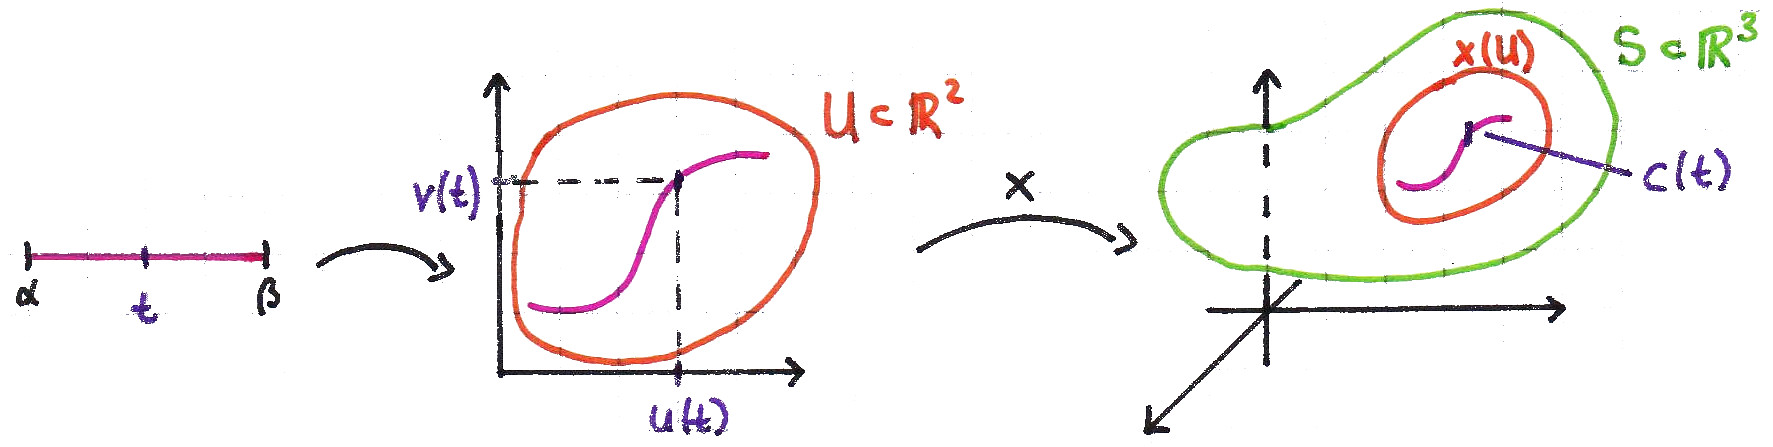
\includegraphics[width=.8\textwidth]{EntstehungFlaechenkurve}
    \caption{Entstehung der Flächenkurve}
  \end{figure}

  \item \emph{Winkel}: Außer Längen können auch Winkel zwischen Flächenkurven als Winkel zwischen den entsprechenden Tangenten an diese Kurven gemessen werden: \\
  Seien \( c_1: (-\epsilon, \epsilon) \to S \), \( c_2: (-\epsilon, \epsilon) \to S \) zwei Flächenkurven mit \( c_1(0) = c_2(0) \).
  \begin{equation*}
    \cos \measuredangle (c_1'(0),c_2'(0)) \coloneqq \frac{\langle c_1'(0), c_2'(0) \rangle}{\Vert c_1'(0) \Vert * \Vert c_2'(0) \Vert}
  \end{equation*}
  Explizite Rechnung via Parametrisierung:
  \begin{align*}
    c_1'(0) &= x_u(u_0, v_0)a + x_v(u_0,v_0)b \\
    c_2'(0) &= x_u(u_0, v_0)c + x_v(u_0,v_0)d
  \end{align*}
  für \( a,b,c,d \in \R \).
  \begin{align*}
    \cos \measuredangle (c_1'(0), c_2'(0)) &= \frac{\langle {x_u}a + {x_v}b, {x_u}c + {x_v}d \rangle}{\Vert {x_u}a + {x_v}b \Vert * \Vert {x_u}c + {x_v}d \Vert} \\
     &= \frac{acE + (bc + ad)F + bdG}{\sqrt{a^2E + 2abF + b^2G}\sqrt{c^2E + 2cdF + d^2G}}
  \end{align*}
  also ist der Winkel zwischen Flächenkurven die Größe des Winkels zwischen zwei Geraden.

  \begin{figure}[H]
    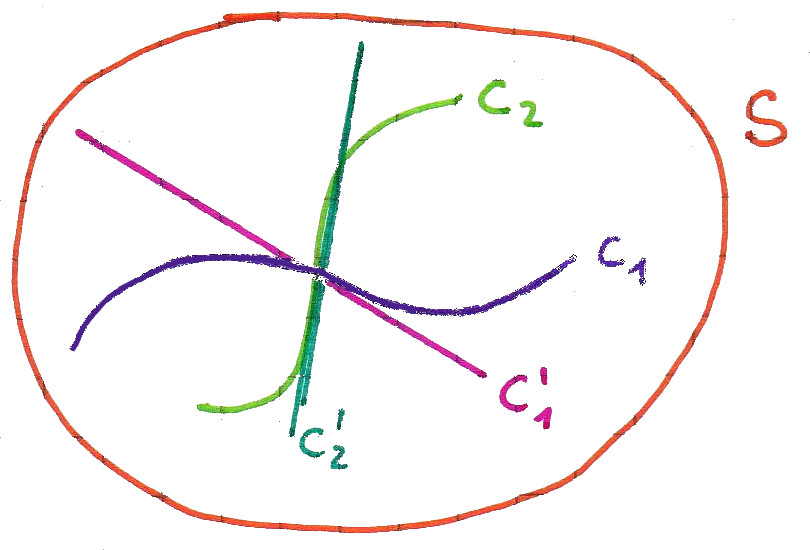
\includegraphics[width=.4\textwidth]{FlaechenkurveTangenten}
    \caption{Zwei Flächenkurven mit dazugehörigen Tangenten}
  \end{figure}

  \item \emph{Flächeninhalt} eines regulären parametrisierten Flächenstücks
  \begin{equation*}
    x(U) \subset S \subset \R^2
  \end{equation*}
  ist definiert als
  \begin{equation*}
    A(x(U)) \coloneqq \iint_U \Vert x_u \wedge x_v \Vert (u,v) \ \text{d}u\text{d}v\text{.}
  \end{equation*}
  Da \( \Vert x_u \wedge x_v \Vert^2 = \langle x_u, x_u \rangle \langle x_v,x_v \rangle - \langle x_u, x_v \rangle^2 = EG - F^2 = \det(\underset{\mathclap{\text{aus 1. FF}}}{I}) \) laut der Formel für das Vektorprodukt (Fläche Parallelogramm im Quadrat) ist \( A \) invariant unter Parameter-Transformationen (also wohldefiniert): \\
  Denn für eine andere Parametrisierung \( \overline{x}: \R^2 \supset \overline{U} \to \overline{x}(\overline{U}) = x(U) \subset S \subset \R^3 \) gilt:
  \begin{equation*}
    I = D^\top \overline{I} D
  \end{equation*}
  wobei \( D = \) Funktionalmatrix des Kartenwechsels (\( = \) Parameter-Transformation \( \overline{x} \circ x^{-1} : U \to \overline{U} \)). Somit:
  \begin{equation*}
    \det(I) = {\left( \det D \right)}^2 \det \overline{I} \quad (\star)
  \end{equation*}
  und die Behauptung folgt aus der Transformationsformel für Integrale:
  \begin{equation*}
    \iint_{\overline{U}} \sqrt{\det \overline{I}} \ \text{d}\overline{u}\text{d}\overline{v} \underset{\mathclap{\text{TF}}}{=} \iint_U \sqrt{\det \overline{I}} \ \vert \det D \vert \ \text{d}u\text{d}v \underset{\mathclap{(\star)}}{=} \iint_U \sqrt{\det I} \ \text{d}u\text{d}v
  \end{equation*}
 \end{enumerate}
\end{remark}

\begin{example}[Beispiel zur Flächeninhaltsberechnung]
  \( S = S_R^2 = \) Sphäre vom Radius \( S \) parametrisiert durch geographische Koordinaten \( (\theta, \phi) \). \\
  Erste Fundamentalform:
  \begin{align*}
    I(\theta, \phi) &= \begin{pmatrix}
    R^2 & 0 \\
    0 & R^2\cos^2 \theta
  \end{pmatrix} \\
  U &= (-\frac{\pi}{2}, \frac{\pi}{2}) \times (0, 2\pi)\text{,}
  \end{align*}
  also
  \begin{align*}
    A(x(U)) &\underset{\mathclap{\substack{x(U) \text{: die} \\ \text{ganze Sphäre bis auf} \\ \text{``Nullmengen'' überdeckt}}}}{=} A(S_R^2) = \iint_U \sqrt{\det I} \ \text{d}\theta \text{d}\phi = \int_{-\frac{\pi}{2}}^{\frac{\pi}{2}} \int_0^{2\pi} R^2\cos \theta \ \text{d}\phi\text{d}\theta \\
     &= R^2 2\pi \int_{-\frac{\pi}{2}}^{\frac{\pi}{2}} \cos \theta \ \text{d}\theta \\
     &= 4 \pi R^2
  \end{align*}
\end{example}

\section{(Lokale) Isometrien von Flächen}

\begin{remark}[Reguläre Fläche = Metrischer Raum]
  Sei \( S \subset \R^3 \) eine reguläre Fläche. Wir definieren eine \emph{Längenmetrik} auf \( S \) durch
  \begin{equation*}
    d_S(p,q) = \underset{\mathclap{\substack{c \in \Omega_{pq}}}}{\text{inf}L(c)}
  \end{equation*}
  mit \( p,q \in S \), \( \Omega_{pq} \coloneqq \) Menge von differenzierbaren \emph{Flächenkurven}, die \( p \) und \( q \) verbinden, \( L(c) \coloneqq \) Länge von \( x \) (gemessen in \( S \)).
  \\
  Wir verifizieren die Metrik-Axiome:
  \begin{itemize}
    \item \( d_S(p,q) = d_S(q,p) \) (Wege rückwärts durchlaufen):
    \begin{equation*}
       c: [0,1] \to S \leadsto \tilde{c}: [0,1] \to S, \ t \mapsto \tilde{c}(t) = c(1-t)
     \end{equation*} 
     \begin{equation*}
       c(0) = p, \ c(1) = q, \quad \tilde{c}(0) = c(1) = q, \ \tilde{c}(1) = p
     \end{equation*}
     und \( L(c) = L(\tilde{c}) \).

    \item \( d_S(p,q) \leq d_S(p,r) + d_S(r,q) \)
    \item \( d_S(p,p) = 0 \): \( c_0(t) = p \leadsto c_0'(t) = 0 \leadsto L(c_0) = 0 \).
  \end{itemize}
  Die obigen Punkte gelten ganz allgemein und haben mit \( S \) nichts zu tun.
  \begin{itemize}
    \item \( p \neq q \Rightarrow d_S(p,q) > 0 \):
    \begin{equation*}
       \exists \ \epsilon > 0 \underset{\text{Def.}}{:} \underset{\epsilon\text{-Bälle in } \R^3}{B_\epsilon(p) \cap B_\epsilon(q)} \cap S = \varnothing\text{.}
     \end{equation*} 
     Hier benutzt man, dass \( \R^3 \) mit Standard-Metrik hausdorffsch ist. Also
     \begin{equation*}
       d_S(p,q) \geq d_{\R^3}(p,q) \geq 2\epsilon > 0\text{.}
     \end{equation*}
  \end{itemize}
  \emph{Fazit}: Jede reguläre Fläche ist metrischer Raum.
\end{remark}

\begin{definition}
  Seien \( S \) und \( \tilde{S} \) reguläre Flächen in \( \R^3 \) und \( f: S \to \tilde{S} \) eine Abbildung.
  \begin{enumerate}

    \item \( f \) heißt \term{(Flächen-)Isometrie}, wenn \( f \) ein Diffeomorphismus von \( S \) auf \( \tilde{S} \) ist und für alle differenzierbaren Kurven \( c: I \to S \) gilt:
    \begin{equation*}
      L(f \circ c) = L(c) \quad \text{``\( f \) ist Längen-erhaltend''.}
    \end{equation*}

    \item \( f \) heißt \term{lokale Isometrie}, falls für jeden Punkt \( p \in S \) offene Umgebungen \( A \) von \( p \) und \( B \) von \( f(p) \) existieren, so dass \( f \) eine Isometrie von \( A \) auf \( B \) ist.
  \end{enumerate}
\end{definition}

\begin{remark}[Abstandserhaltend]
  Ist \( f: S \to \tilde{S} \) eine Flächen-Isometrie, so ist \( f \) eine Isometrie zwischen den metrischen Räumen \( (S, d_S) \) und \( (\tilde{S}, d_{\tilde{S}}) \), also gilt:
  \begin{equation*}
    \forall p,q \in S : d_{\tilde{S}}(f(p),f(q)) = d_S(p,q) \quad \text{``\( f \) ist Abstands-erhaltend''.}
  \end{equation*}
\end{remark}

\begin{theorem}[Kriterium für lokale Isometrien]
  Sind \( S \) und \( \tilde{S} \) reguläre Flächen und sind \( x: U \to x(U) \subset S \) und \( \tilde{x}: U \to \tilde{x}(U) \subset \tilde{S} \) mit \textbf{gleichem} Parameterbereich \( U \), sodass
  \begin{equation*}
    \forall (u,v) \in U : \underset{\text{1. FF von } S}{\begin{pmatrix}
      E & F \\
      F & G
    \end{pmatrix}}(u,v) = \underset{\text{1. FF von } \tilde{S}}{\begin{pmatrix}
      \tilde{E} & \tilde{F} \\
      \tilde{F} & \tilde{G}
    \end{pmatrix}}(u,v)\text{,}
  \end{equation*}
  das heißt: Stimmen die erste Fundamentalform von \( S \) und \( \tilde{S} \) in entsprechenden Punkten überein, so sind \( x(U) \) und \( \tilde{x}(U) \) isometrisch.
  \begin{proof}
    Die Abbildung \( f \coloneqq \tilde{x} \circ x^{-1}: S \supset x(U) \to \tilde{x}(U) \subset \tilde{S} \) ist Diffeomorphismus. Sei dann
    \begin{equation*}
      c: [a,b] \to S, \ c(t) = x(u(t),v(t)) \subset x(U) \subset S
    \end{equation*}
    eine differenzierbare (Test-)Kurve. \\
    Dann gilt:
    \begin{align*}
      L(c) &= \int_a^b \Vert c'(t) \Vert \ \text{d}t \\
      &= \int_a^b \sqrt{E^2(u(t),v(t)){(u')}^2 + 2F(u(t),v(t))u'v' + G^2(u(t),v(t)){(v')}^2} \ \text{d}t \\
      &\underset{\mathclap{\text{Vorr.}}}{=} \int_a^b \sqrt{\tilde{E}(u(t),v(t)){(u')}^2 + 2u'v'\tilde{F}(u(t),v(t)) + {(v')}^2\tilde{G}(u(t),v(t))} \ \text{d}t\text{.}
    \end{align*}
    Andererseits gilt für die Länge der Bildkurve
    \begin{equation*}
      f \circ c(t) = (\tilde{x} \circ x^{-1}) \circ x(u(t),v(t)) = \tilde{x}(u(t),v(t))\text{:}
    \end{equation*}
    \begin{equation*}
      L(f \circ c) = \int_a^b \sqrt{\tilde{E}(u(t),v(t)){(u')}^2 + 2u'v' \tilde{F}(u(t),v(t)) + {(v')}^2\tilde{G}(u(t),v(t))} \ \text{d}t\text{.}
    \end{equation*}
    \qed{}
  \end{proof}
\end{theorem}

\begin{figure}[H]
  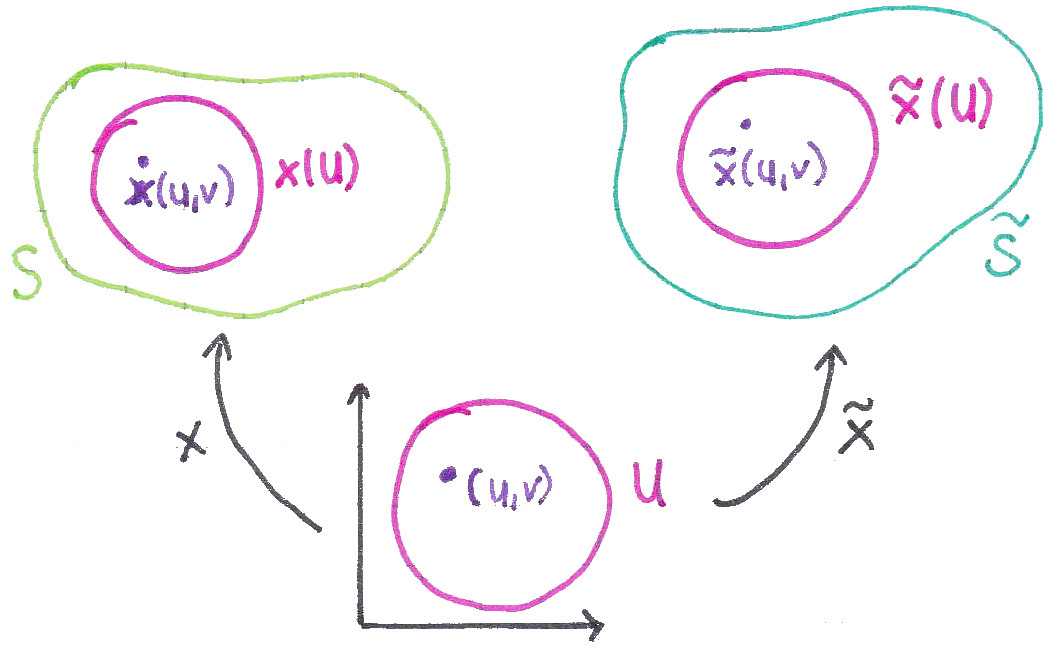
\includegraphics[width=.5\textwidth]{LokalIsometrisch}
  \caption{\( x(U) \) und \( \tilde{x}(U) \) sind isometrisch}
\end{figure}

\section{Normalvektoren und zweite Fundamentalform}

Ist \( S \) reguläre Fläche in \( \R^3 \), dann existiert in jedem Punkt \( p \in S \) die Tangentialebene. Für gegebene Parametrisierung 
\begin{equation*}
  x : U \ni (u,v) \mapsto x(u,v) \in S
\end{equation*}
um \( p \) ist \( T_p S = [x_u,x_v] \). \\
Ist \( \overline{x} : \overline{U} \to S \) eine andere Parametrisierung um \( p \in S \), so gilt: \( [\overline{x}_{\overline{u}},\overline{x}_{\overline{v}}] = [x_u,x_v] \). \\
Weiter gilt für das Vektorprodukt:
\begin{align*}
  \overline{x}_{\overline{u}} \wedge \overline{x}_{\overline{v}} &= \left( x_u\frac{\partial u}{\partial \overline{u}} + x_v\frac{\partial v}{\partial \overline{u}} \right) \wedge \left( x_u\frac{\partial u}{\partial \overline{v}} + x_v\frac{\partial v}{\partial \overline{v}} \right) \\
  &= \left( \frac{\partial u}{\partial \overline{u}}*\frac{\partial v}{\partial \overline{v}} - \frac{\partial u}{\partial \overline{v}}*\frac{\partial v}{\partial \overline{u}} \right) (x_u \wedge x_v) \\
  &= \det(\text{d}\phi)(x_u \wedge x_v)\text{,}
\end{align*}
wobei \( \phi = x^{-1} \circ \overline{x} : \overline{U} \to U \) die Koordinatentransformation (Parameterwechsel) und \( \text{d}\phi \) das Differential davon ist.

\begin{definition}[Normalenvektor]
  Da \( x_u \) und \( x_v \) linear unabhängig sind, ist
  \begin{equation*}
    x_v \wedge x_u \neq 0 \quad \text{und} \quad n(p) \cong n(x(u,v)) \equiv n(u,v) \coloneqq \frac{x_u(u,v) \wedge x_v(u,v)}{\Vert x_u(u,v) \wedge x_v(u,v) \Vert}
  \end{equation*}
  ist ein Einheitsvektor senkrecht zu \( T_p S \) für alle \( p \in x(U) \subset S \). \\
  \( n(p) \) heißt \term{Normalenvektor}\label{def:normalenvektor} von \( S \) im Punkt \( p \). \\
  Nach obiger Rechnung gilt für eine andere Parametrisierung um \( p \):
  \begin{align*}
    \overline{n}(p) = \frac{\overline{x}_{\overline{u}} \wedge \overline{x}_{\overline{v}}}{\Vert \overline{x}_{\overline{u}} \wedge \overline{x}_{\overline{v}} \Vert} = \frac{\det(\text{d}\phi)x_u \wedge x_v}{\vert \det(\text{d}\phi) \vert * \Vert x_u \wedge x_v \Vert} = \frac{\det(\phi)}{\vert \det(\phi) \vert} n(p) = \pm n(p)
  \end{align*}
  Damit die Normalenvektoren eindeutig bestimmt sind, brauchen wir die Voraussetzung, dass \( \det(\text{d}\phi) > 0 \) für alle Parameterwechsel.
\end{definition}

\begin{definition}[Orientierbarkeit]
  Eine reguläre Fläche \( S \) --- oder allgemeiner, eine differenzierbare Mannigfaltigkeit \( M \) --- heißt \term{orientierbar}\label{def:orientierbarkeit}, falls ein Atlas von \( S \) (bzw. \( M \)) existiert, sodass alle Kartenwechsel (Parameterwechsel) eine positive Funktionaldeterminante haben.
\end{definition}

\begin{example}[Orientierbarkeit von Flächen]
  Sphären und Tori sind orientierbar, Möbiusband und projektive Ebene nicht.
\end{example}

\begin{example}[Normalenvektoren]
  \
  \begin{enumerate}
    \begin{minipage}{.575\textwidth}
      \item \textbf{Affine Ebene}: \( x(u,v) = ua + vb \), \( a \), \( b \) linear unabhängig \\
        \( \to \ x_u = a \), \( x_v = b \), \( n(p) = \frac{x_u \wedge x_v}{\Vert x_u \wedge x_v \Vert} = \frac{a \wedge b}{\Vert a \wedge b \Vert} = \) konstant
    \end{minipage}
    \hfill
    \begin{minipage}{.375\textwidth}
      \begin{figure}[H]
        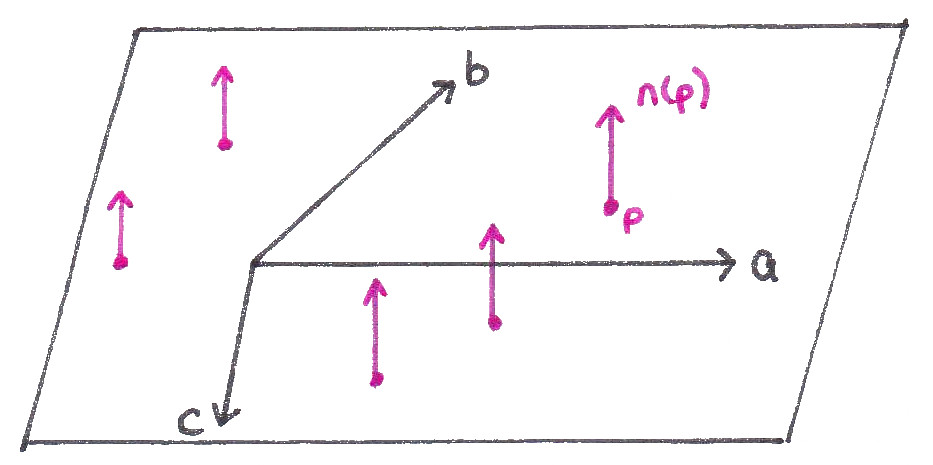
\includegraphics[width=.9\textwidth]{AffineEbeneNormalenvektoren}
        \caption{Affine Ebene mit Normalenvektoren}
      \end{figure}
    \end{minipage}
    \item \textbf{2-Sphäre \( S^2 \) mit Radius \( R \)}:
      \begin{align*}
        x(\theta, \phi) &= \left( \begin{smallmatrix}
          R\cos\theta\cos\phi \\
          R\cos\theta\sin\phi \\
          R\sin\theta
        \end{smallmatrix} \right), \enskip x_\theta = \left( \begin{smallmatrix}
          -R\sin\theta\cos\phi \\
          -R\sin\theta\sin\phi \\
          R\cos\theta
        \end{smallmatrix} \right), \enskip x_\phi = \left( \begin{smallmatrix}
          -R\cos\theta\sin\phi \\
          R\cos\theta\cos\phi \\
          0
        \end{smallmatrix} \right) \\
        x_\theta \wedge x_\phi &= \left( \begin{smallmatrix}
          -R^2\cos^2\theta\cos\phi \\
          -R^2\cos^2\theta\sin\phi \\
          R\sin\theta\cos\theta
        \end{smallmatrix} \right) = -R\cos\theta \left( \begin{smallmatrix}
          R\cos\theta\cos\phi \\
          R\cos\theta\sin\phi \\
          R\sin\phi
        \end{smallmatrix} \right) = -R\cos\theta x(u,v) \\
        n(\theta, \phi) &\coloneqq \frac{x_\theta \wedge x_\phi}{\Vert x_\theta \wedge x_\phi \Vert} = \frac{-x(\theta, \phi)}{\Vert x(\theta,\phi) \Vert} \quad \text{(``innere Normale'')} \\
        \overline{n}(\theta,\phi) &\coloneqq \frac{x_\phi \wedge x_\theta}{\left\Vert x_\phi \wedge x_\theta \right\Vert} = - n(\theta,\phi) \quad \text{(``äußere Normale'')}
      \end{align*}
  \end{enumerate}
\end{example}

\begin{figure}[H]
  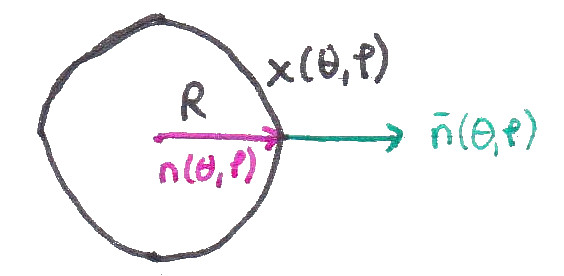
\includegraphics[width=0.4\textwidth]{Normalen2Sphaere}
  \caption{Äußere und innere Normale an der \( 2 \)-Sphäre}
\end{figure}

\begin{remark}[Krümmungsmessung]
  Frage: Wie soll man Krümmung messen? \\
  Möglichkeit nach Gauß: ``Änderung der Normalen'' messen --- wie ändert sich die Normale, wenn \( p \in S \) sich ändert? \\
  Betrachte eine Testkurve auf \( S \): \( c(t) = x(u(t),v(t)) \) und Normalenvektoren von \( S \) entlang \( c(t) \): \( n(c(t)) \). Dann ergibt sich die Änderung:
  \begin{align*}
    \frac{\text{d}}{\text{d}t}n(c(t)) &= \frac{\text{d}}{\text{d}t}n(u(t),v(t)) = \frac{\partial n}{\partial u}\frac{\partial u}{\partial t} + \frac{\partial n}{\partial v}\frac{\partial v}{\partial t} \\
    &= n_u \frac{\partial u}{\partial t} + n_v \frac{\partial v}{\partial t} = {n_u}u' + {n_v}v'
  \end{align*}
\end{remark}

\begin{figure}[H]
  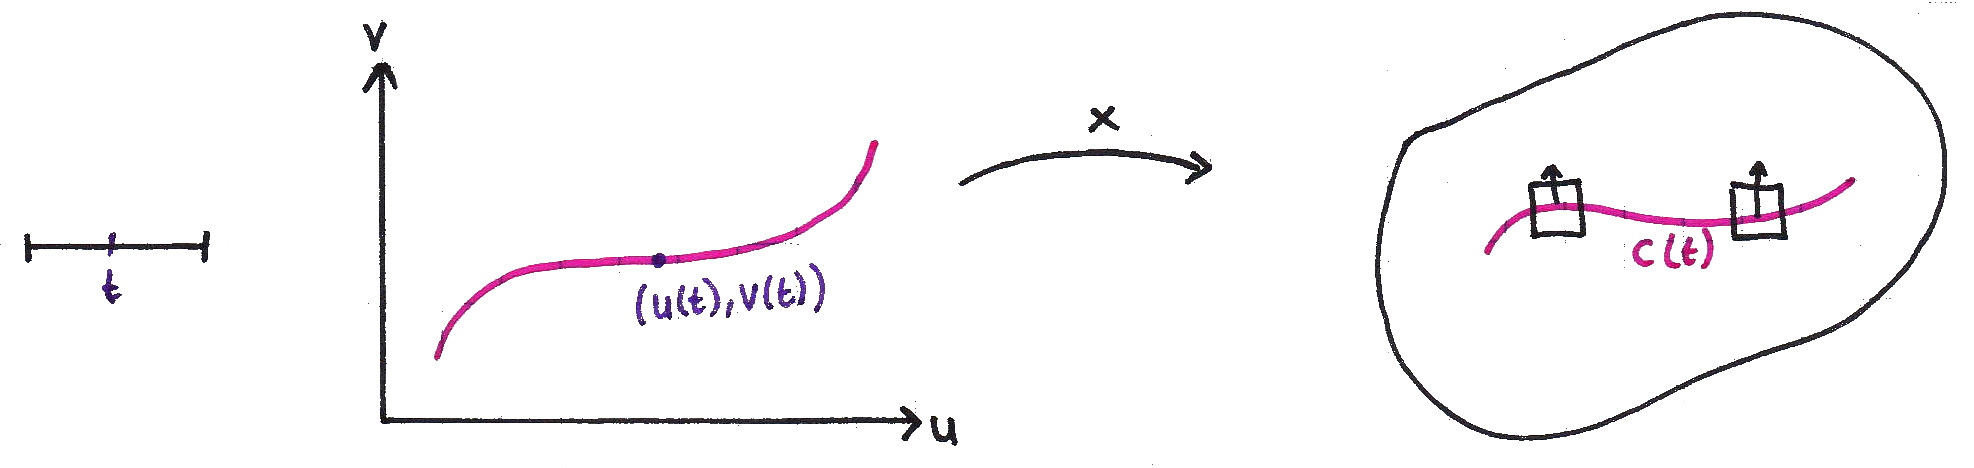
\includegraphics[width=\textwidth]{Kruemmungsmessung}
\end{figure}

\begin{remark}[Zwischenbemerkung]
  Für differenzierbare Kurven \( a(t) \), \( b(t) \) in \( \R^3 \) gilt:
  \begin{align*}
    \frac{\text{d}}{\text{d}t}\langle a(t), b(t) \rangle &= \frac{\text{d}}{\text{d}t}\left( a_1(t)b_1(t)+a_2(t)b_2(t)+a_3(t)b_3(t) \right) \\
     &= a_1'b_1+a_1b_1'+a_2'b_2+a_2b_2' + a_3'b_3+a_3b_3' \\
     &= \langle a'(t),b(t) \rangle + \langle a(t),b'(t) \rangle = \langle \frac{\text{d}}{\text{d} t}a(t),b(t) \rangle + \langle a(t), \frac{\text{d}}{\text{d}t}b(t) \rangle\text{.}
  \end{align*}
  Es ist \( \langle n(t),n(t) \rangle = \Vert n(t) \Vert^2 = 1 \), also
  \begin{align*}
    \langle n_u,n \rangle &= \frac{1}{2}\frac{\text{d}}{\text{d}u}\langle n,n \rangle = 0 \\
    \text{und } \langle n_v,n \rangle &= \frac{1}{2}\frac{\text{d}}{\text{d}v}\langle n,n \rangle = 0\text{.}
  \end{align*}
  \( n_u \) ist also durch die Komponenten des Skalarprodukts bestimmt:
  \begin{equation*}
    \langle n_u,x_u \rangle = -\langle n,x_{uu} \rangle \quad \text{und} \quad \langle n_u,x_v \rangle = - \langle n,x_{uv} \rangle
  \end{equation*}
  wobei
  \begin{equation*}
    x_{uu} \coloneqq \frac{\text{d}^2x}{\text{d}u^2}, \quad x_{uv}= \frac{\text{d}^2x}{\text{d}u\text{d}v} = \frac{\text{d}^2x}{\text{d}v\text{d}u} = x_{vu}
  \end{equation*}
\end{remark}

Diese Formeln motivieren folgende Definition:

\begin{definition}[2. Fundamentalform]
  Die \term{2. Fundamentalform}\label{def:zweiteFundamentalform} einer regulären (orientierbaren) Fläche \( S \) ist eine Familie von Bilinearformen \( \left \{ \rom{2}_p : p \in S \right \} \), die für eine Parametrisierung \( x: U \to S \) (bezüglich der Basen \( \{ x_u, x_v \} \) von \( T_{x(u,v)}S \)) gegeben ist durch die symmetrischen Matrizen:
  \begin{equation*}
    \begin{pmatrix}
      L(u,v) & M(u,v) \\
      M(u,v) & N(u,v)
    \end{pmatrix} \coloneqq \begin{pmatrix}
      \langle x_{uu},n \rangle & \langle x_{uv},n \rangle \\
      \langle x_{vu},n \rangle & \langle x_{vv},n \rangle
    \end{pmatrix}
  \end{equation*}
  \textbf{Hinweis}: \( \rom{2}_p \) ist symmetrisch, aber im Allgemeinen \underline{nicht} positiv definit.
\end{definition}

\begin{example}[zur zweiten Fundamentalform]
  \
  \begin{enumerate}
    \item \emph{Ebene}: \( x_u = a \), \( x_v = b \), \( x_{uu} = 0 \), \( x_{ uv } = 0 \), \( x_{ vv } = 0 \). \\
      Also ist \( \rom{2}_p = 0 \) für alle \( p \in S \cong \) Ebene.
    \item \emph{Zylinder}:
    \begin{align*}
      x(u,v) &= \left( \begin{smallmatrix}
        r\cos u \\ r\sin u \\ v
      \end{smallmatrix} \right), \ x_u = \left( \begin{smallmatrix}
        -r\sin u \\ r\cos u \\ 0
      \end{smallmatrix} \right), \ x_v = \left( \begin{smallmatrix}
        0 \\ 0 \\ 1
      \end{smallmatrix} \right), \\
      x_{uu} &= \left( \begin{smallmatrix}
        -r\cos u \\ -r\sin u \\ 0
      \end{smallmatrix} \right), \ x_{uv} = x_{vu} = x_{vv} = \left( \begin{smallmatrix}
         0 \\ 0 \\ 0
      \end{smallmatrix} \right)\text{, also}
    \end{align*}
    \begin{equation*}
      \rom{2}_{x(u,v)} = \begin{pmatrix}
        -r & 0 \\
        0 & 0
      \end{pmatrix}\text{.}
    \end{equation*}
  \end{enumerate}
\end{example}

\section{Gauß-Krümmung}

\begin{definition}[Gauß-Krümmung]
  Sei \( S \) eine reguläre Fläche, \( p \in S \). Die \term{Gauß-Krümmung}\label{def:gaussKruemmung} von \( S \) ist die Funktion
  \begin{equation*}
    \kappa: S \ni p \mapsto \kappa(p) \coloneqq \frac{\det \rom{2}_p}{\det \rom{1}_p} \in \R
  \end{equation*}
\end{definition}

\begin{remark}[Invarianz Gauß-Krümmung]
  \( \kappa \) ist invariant unter Parameterwahl.
  \begin{proof}
    Seien \( x \), \( \overline{x} \) lokale Parametrisierungen von \( S \) um \( p \in S \). Sei \( \phi \coloneqq \overline{x}^{-1} \circ x \) der Parameterwechsel.
    \begin{align*}
      \rom{1}_p &= \left( \begin{smallmatrix}
        \langle x_u,x_u \rangle & \langle x_u,x_v \rangle \\
        \langle x_v,x_u \rangle & \langle x_v,x_v \rangle
      \end{smallmatrix} \right) = J_x^\top J_x \\
      \rom{2}_p &= \left( \begin{smallmatrix}
        \langle x_{uu}, n \rangle & \langle x_{uv}, n \rangle \\ 
        \langle x_{vu}, n \rangle & \langle x_{vv}, n \rangle
      \end{smallmatrix} \right) = -J_x^\top J_n
    \end{align*}
    Es ist \( J_x = J_{\overline{x} \circ \phi} = J_{\overline{x}}J_\phi \), \( J_n = J_{\overline{n} \circ \phi} = J_{\overline{n}}J_\phi \), also ist
    \begin{align*}
      \rom{1}_p &= J_x^\top J_x = {(J_{\overline{x}}J_\phi)}^\top J_{\overline{x}}J_\phi = J_\phi^\top J_{\overline{x}}^\top J_{\overline{x}} J_\phi = J_\phi^\top \overline{\rom{1}}_p J_\phi \\
      \rom{2}_p &=- J_x^\top J_n = \cdots = J_\phi^\top \overline{\rom{2}}_p J_\phi
    \end{align*}
    und damit
    \begin{equation*}
      \frac{\det \rom{2}_p}{\det \rom{1}_p} = \frac{\det \overline{\rom{2}}_p}{\det \overline{\rom{1}}_p}
    \end{equation*} \qed{}
  \end{proof}
\end{remark}

\begin{example}[Gauß-Krümmung]
  \
  \begin{enumerate}
    \item \emph{Fläche}:
    \begin{align*}
      x(u,v) &= \left( \begin{smallmatrix}
        u \\ v \\ 0
      \end{smallmatrix} \right), \ x_u = \left( \begin{smallmatrix}
        1 \\ 0 \\ 0
      \end{smallmatrix} \right), \ x_v = \left( \begin{smallmatrix}
        0 \\ 1 \\ 0
      \end{smallmatrix} \right) \\
      x_u \wedge x_v &= \left( \begin{smallmatrix}
        0 \\ 0 \\ 1
      \end{smallmatrix} \right) = n, \ x_{uu} = x_{uv} = x_{vv} = 0
    \end{align*}
    Also ist
    \begin{equation*}
      \rom{1} = \begin{pmatrix}
        1 & 0 \\
        0 & 1
      \end{pmatrix}, \quad \rom{2} = \begin{pmatrix}
        0 & 0 \\
        0 & 0
      \end{pmatrix} \quad \Rightarrow \kappa = 0\text{.}
    \end{equation*}

    \item \emph{Zylinder}:
    \begin{align*}
      x(u,v) &= \left( \begin{smallmatrix}
      r\cos u \\ r\sin u \\ v
    \end{smallmatrix} \right), \ x_u = \left( \begin{smallmatrix}
      -r\sin u \\ r\cos u \\ 0
    \end{smallmatrix} \right), \ x_v = \left( \begin{smallmatrix}
      0 \\ 0 \\ 1
    \end{smallmatrix} \right), \\
    x_u \wedge x_v &= \left( \begin{smallmatrix}
      r\cos u \\
      r\sin u \\
      0
    \end{smallmatrix} \right), n = \left( \begin{smallmatrix}
      \cos u \\ \sin u \\ 0
    \end{smallmatrix} \right), x_{uu} = \left( \begin{smallmatrix}
      -r\cos u \\ -r\sin u \\ 0
    \end{smallmatrix} \right), x_{uv} = x_{vv} = 0
    \end{align*}
    Also ist
    \begin{equation*}
      \rom{1} = \begin{pmatrix}
        r^2 & 0 \\
        0 & \cos^2(u)r^2
      \end{pmatrix}, \quad \rom{2} = \begin{pmatrix}
        -r & 0 \\
        0 & 0
      \end{pmatrix} \quad \Rightarrow \kappa = 0\text{.}
    \end{equation*}

    \item \emph{Kugel}: \( (u,v) \in \left( -\tfrac{\pi}{2}, \tfrac{\pi}{2} \right) \times (0, 2\pi) \),
    \begin{align*}
      x(u,v) &= \left( \begin{smallmatrix}
      r\cos u \cos v \\ r\cos u \sin v \\ r\sin u
    \end{smallmatrix} \right), \ x_u = \left( \begin{smallmatrix}
      -r\sin u \cos v \\ -r\sin u \sin v \\ r\cos u
    \end{smallmatrix} \right), \ x_v = \left( \begin{smallmatrix}
      -r\cos u \sin v \\ r\cos u \cos v \\ 0
    \end{smallmatrix} \right) \\
    \Rightarrow x_u \wedge x_v &= -r^2\cos u \left( \begin{smallmatrix}
      \cos u \cos v \\ \cos u \sin v \\ \sin u
    \end{smallmatrix} \right), \ n = \left( \begin{smallmatrix}
      -\cos u \cos v \\ -\cos u \sin v \\ -\sin u
    \end{smallmatrix} \right), \\
    x_{uu} &= \left( \begin{smallmatrix}
      -r\cos u\cos v \\ -r\cos u \sin v \\ -r\sin u
    \end{smallmatrix} \right) = -x, \ x_{uv} = \left( \begin{smallmatrix}
      r\sin u \sin v \\ -r\sin u \cos v \\ 0
    \end{smallmatrix} \right), \ x_{vv} = \left( \begin{smallmatrix}
      -r\cos u \cos v \\ -r\cos u \sin v \\ 0
    \end{smallmatrix} \right)\text{.}
    \end{align*}
    Also ist
    \begin{equation*}
      \rom{1} = \begin{pmatrix}
        r^2 & 0 \\
        0 & \cos^2(u)r^2
      \end{pmatrix}, \quad \rom{2} = \begin{pmatrix}
        r & 0 \\
        0 & \cos^2(u)r^2
      \end{pmatrix}, \quad \Rightarrow \kappa = \frac{r^3\cos^2 u}{r^4\cos^2 u} = \frac{1}{r}
    \end{equation*}

  \end{enumerate}
\end{example}

\begin{theorem}[theorem egregium, Gauß 1827]
  Die Gauß-Krümmung \( \kappa \) einer regulären Fläche \( S \) ist eine Größe der inneren Geometrie von \( S \), also kann \( \kappa \) aus den Funktionen \( E \), \( F \) und \( G \) beziehungsweise deren Ableitungen berechnet werden.
\end{theorem}

\begin{theorem}[Satz von Bertrand-Puiseux, 1848]
  \

  \begin{minipage}{.625\textwidth}
    Sei \( S \) eine reguläre Fläche und \( p \in S \). Für hinreichend kleine \( r > 0 \) ist
    \begin{equation*}
      S_r(p) \coloneqq \{ q \in S : d(p,q) = r \}
    \end{equation*}
    eine geschlossene, differenzierbare Kurve der Länge \( L(S_r(p)) \). Dann gilt:
    \begin{equation*}
      \kappa(p) = \lim_{r \to 0} \frac{3}{\pi r^3}(2\pi r - L(S_r(p)))\text{.}
    \end{equation*}
  \end{minipage}
  \hfill
  \begin{minipage}{.35\textwidth}
    \begin{figure}[H]
      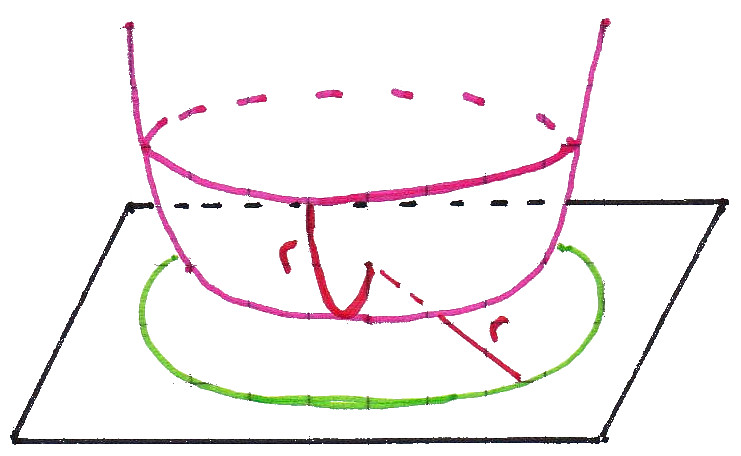
\includegraphics[width=.8\textwidth]{BertrandPuiseux}
    \end{figure}
  \end{minipage}
\end{theorem}

\section{Der Satz von Gauß-Bonnet --- lokale Version}

\begin{definition}[Kovariante Ableitung]
  Gegeben sei eine lokale Parametrisierung \( x: U \to S \). Sei \( a : U \to \R^3 \) ein tangentiales Vektorfeld auf \( S \), also
  \begin{equation*}
    a(u,v) \in T_{x(u,v)}S \quad \forall (u,v) \in U\text{.}
  \end{equation*}
  Insbesondere ist \( a \perp n \). \\
  Im Allgemeinen ist \( a_u(u,v) \coloneqq \frac{\partial a(u,v)}{\partial u} \not \in T_{x(u,v)}S \), daher definiert man die \term{kovariante Ableitung}\label{def:kovarianteAbleitung} von \( a \) nach \( u \) als
  \begin{equation*}
    D_u a \coloneqq a_u - \langle n, a_u \rangle n\text{.}
  \end{equation*}
  Dies ist die Komponente von \( a_u \) in Tangentialrichtung, also die Orthogonalprojektion von \( a_u \) auf \( T_{x(u,v)}S \). \\
  Da \( n \perp a \) ist, ist \( \langle n, a \rangle = 0 \), also
  \begin{equation*}
    0 = \frac{\text{d}}{\text{d}u}\langle n,a \rangle = \langle n_u, a \rangle + \langle n, a_u \rangle\text{,}
  \end{equation*}
  also ist
  \begin{equation*}
    D_u a = a_u + \langle n_u, a \rangle n\text{.}
  \end{equation*}
\end{definition}

\begin{definition}[Geodätische Krümmung]
  \  \\
  Sei \( c(s) \coloneqq x(u(s), v(s)) \) eine Flächenkurve, ohne Einschränkung sei \( c \) nach Bogenlänge parametrisiert, also \( \Vert \frac{\partial c}{\partial s} (s) \Vert = 1 \). Nun gilt \( \langle c', c' \rangle = \Vert c' \Vert^2 = 1 \), also ist
  \begin{equation*}
    0 = \frac{\text{d}}{\text{d}s}\langle c', c' \rangle = \langle c'', c' \rangle = \langle c'', c' \rangle + \langle c', c'' \rangle = 2\langle c', c'' \rangle\text{,}
  \end{equation*}
  also ist \( c' \perp c'' \). \( c' \) ist Tangentialvektor, also \( c' \perp n \). \\
  Da \( c' \) und \( n \) orthogonale Einheitsvektoren sind, ist \( \{ c', n \wedge c', n \} \) eine Orthonormalbasis von \( \R^3 \). Bezüglich dieser Basis können wir \( c'' \) jetzt aufspalten:
  \begin{equation*}
    c''(s) = \underset{c'' \perp c'}{0}*c'(s) + \kappa_g(s)(n(s) \wedge c'(s)) + \alpha(s)n(s)\text{.}
  \end{equation*}
  Wir bezeichnen \( \kappa_g(s) \) als \term{geodätische Krümmung}\label{def:geodaetischeKruemmung} von \( c \) in \( c(s) \). \\
  ``Linkskurven'' haben positive geodätische Krümmung, ``Rechtskurven'' negative, wobei ``oben'' durch den Normalenvektor bestimmt wird. \\
  Durchläuft man \( c \) rückwärts, so kehrt sich das Vorzeichen von \( \kappa_g \) um\footnote{siehe Übungsblatt}.
  \begin{figure}[H]
    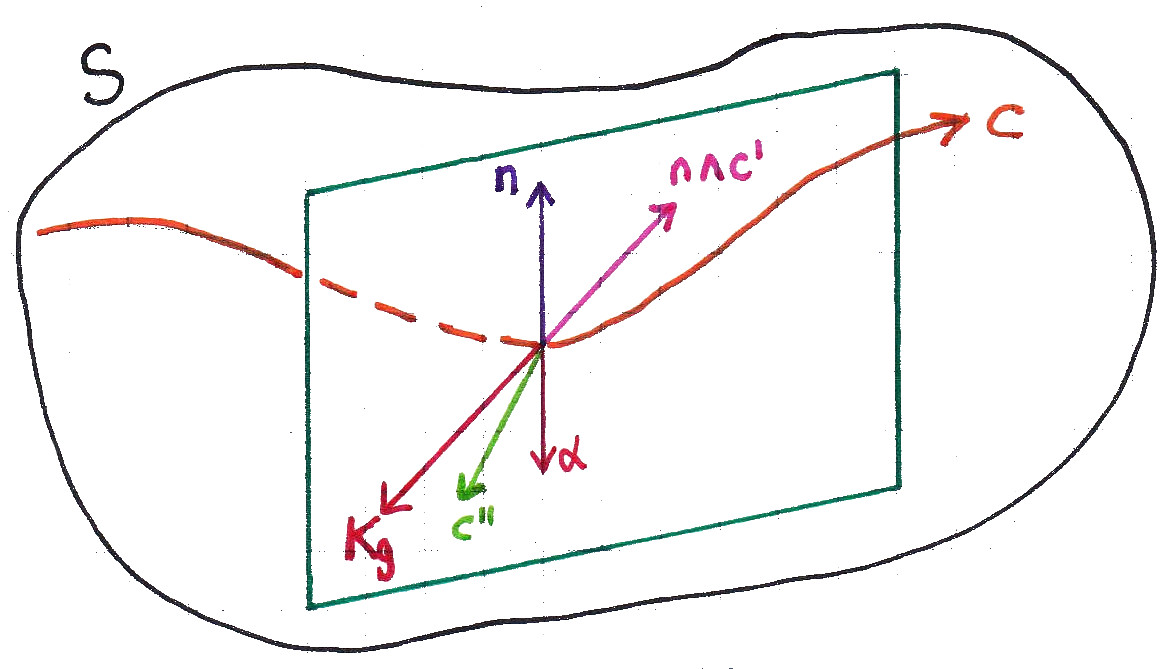
\includegraphics[width=.6\textwidth]{GeodaetischeKruemmung}
    \caption{Geodätische Krümmung von \( c \)}
  \end{figure}
\end{definition}


Es folgen nun einige Lemmata, die als Vorbereitung für den Beweis des Satzes von Gauß-Bonnet benötigt werden.

\begin{lemma}[Formel von Stokes]
  Sei \( \widetilde{G} \) ein ebenes Gebiet mit differenzierbarem Rand \( \delta\widetilde{G} \). Seien \( P,Q : \widetilde{G} \to \R \) differenzierbar. Dann:
  \begin{equation*}
     \landdownint_{\delta(\widetilde{G})}Pu+Qv \text{d}s = \iint_{\widetilde{G}}(Qu-Pv)\text{d}u\text{d}v\text{.}
  \end{equation*} 
  \begin{proof}
    ohne Beweis. \qed{}
  \end{proof}
\end{lemma}

\begin{lemma}
  \
  
  \begin{minipage}{.6\textwidth}
    \begin{enumerate}
      \item Für ein Einheitstangentenvektorfeld
      \begin{equation*}
        e: S \ni p \mapsto e(p) \in T_p S \quad (\text{also } e(p) \in \R^3)
      \end{equation*}
      längs \( S \) gilt:
      \begin{equation*}
        \langle D_u e, e \rangle = 0\text{.}
      \end{equation*}
  
      \item Es ist
      \begin{equation*}
        D_u(\underset{\mathclap{\substack{\text{Normalen-} \\ \text{vektorfeld}}}}{fn}) = fn_u \quad (f: U \to \R \ \ C^\infty)\text{.}
      \end{equation*}
    \end{enumerate}
  \end{minipage}
  \hfill
  \begin{minipage}{.375\textwidth}
    \begin{figure}[H]
      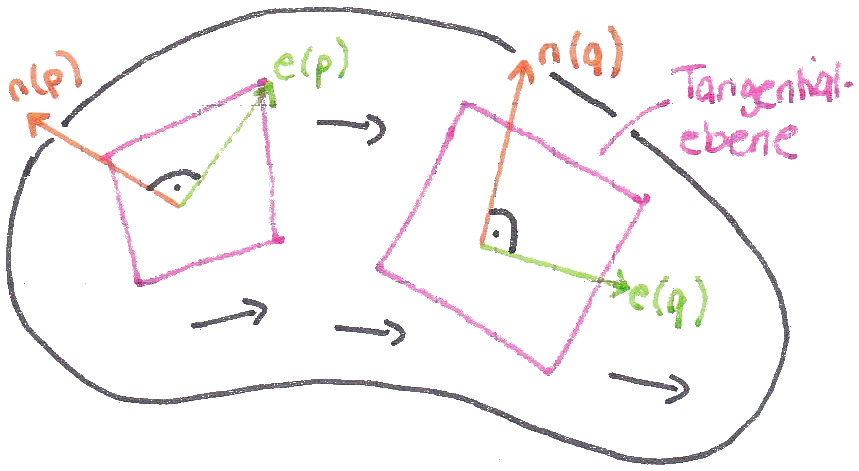
\includegraphics[width=\textwidth]{Einheitstangentenvektorfeld}
    \end{figure}
  \end{minipage}
  \begin{proof}
    \ 
    \begin{enumerate}
      \item Es ist
      \begin{align*}
        \langle e, e \rangle = 1 \Rightarrow \frac{\partial}{\partial u}\langle e, e \rangle &= 0 \\
          &= 2\langle \frac{\partial e}{\partial u}, e \rangle = 2\langle D_u e + \alpha n, e \rangle\text{,}
      \end{align*}
      also \( 0 = \left\langle D_u e,e \right\rangle + \underset{=0}{\left\langle \alpha n, e \right\rangle} = \left\langle D_u e,e \right\rangle = 0 \). \qed{}

      \item Es ist
      \begin{equation*}
        D_u(fn) = {(fn)}_u - \left\langle {(fn)}_u, n \right\rangle n \underset{\mathclap{\substack{\text{Ketten-}\\ \text{regel}}}}{=} \overset{\text{normal}}{f_u n} + \overset{\text{tangential}}{fn_u} - \overset{\text{normal}}{\left\langle {(fn)}_u, n \right\rangle n}\text{.}
      \end{equation*}
      Vergleich der Tangential-Anteile ergibt Behauptung: \( D_u(fn) = fn_u \). \qed{}
    \end{enumerate}
  \end{proof}
\end{lemma}

\begin{lemma}
  Sei \( a: U \to \R^3 \) ein tangentiales Vektorfeld längs \( S \). Dann ist
  \begin{equation*}
    (D_v D_u-D_u D_v)a = (K\sqrt{EG - F^2})(n \wedge a)\text{.}
  \end{equation*}
  \begin{proof}
    \
    \begin{align*}
      D_v D_u a &= D_v(a_u + \left\langle n_u,a \right\rangle n) = D_v a_u + D_v(\left\langle n_u,a \right\rangle n) \\
       &= a_{uv} - \left\langle n,a_{uv} \right\rangle n + D_v(\underbrace{\left\langle n_u,a \right\rangle n}_{=f_1n}) \\
       &\underset{\text{L2}}{=} a_{uv} - \left\langle n,a_{uv} \right\rangle n -f_1n_v \\
       &\Rightarrow (D_v D_u - D_u D_v)a = \underbrace{\left\langle n_v,a \right\rangle n_u}_{f_2 n_u} - \left\langle n_u,a \right\rangle n_v \overset{(\star)}{=} (n_u \wedge n_v)\wedge a\text{.}
    \end{align*}
    \( (\star) \): für \( a,b,c \in \R^3 \) ist \( \left\langle b,a \right\rangle c - \left\langle c,a \right\rangle b = (b \wedge c) \wedge a \). \\ Also ist \( \left\langle a \wedge b, c \wedge d \right\rangle = \left\langle a, c \right\rangle \left\langle b, d \right\rangle - \left\langle a, d \right\rangle \left\langle b, c \right\rangle \). \\
    \  \\
    Es ist \( n_u \wedge n_v = \underset{\in \R}{\lambda}n \), also ist zu zeigen, dass \( \lambda = K\sqrt{EG - F^2} \):
    \begin{align*}
      \left\langle \lambda n, x_u \wedge x_v \right\rangle &= \left\langle n_u \wedge n_v, x_u \wedge x_v \right\rangle \overset{(\star)}{=} \left\langle n_u, x_u \right\rangle \left\langle n_v, x_v \right\rangle - \left\langle n_u, x_v \right\rangle \left\langle n_v,x_u \right\rangle = LN - M^2 \\
      \left\langle n, x_u \wedge x_v \right\rangle &= \left\langle \frac{x_u \wedge x_v}{\left\Vert x_u \wedge x_v \right\Vert}, x_u \wedge x_v \right\rangle = \left\Vert x_u \wedge x_v \right\Vert = \sqrt{EG - F^2}\text{, also} \\
      &\Rightarrow \lambda \sqrt{EG - F^2} = LN - M^2 = \frac{LN - M^2}{EG - F^2}(EG - F^2) = K(EG - F^2)\text{, also} \\
      &\lambda = K\sqrt{EG - F^2}\text{.}
    \end{align*} \qed{}
  \end{proof}
\end{lemma}

\begin{theorem}[Satz von Gauß-Bonnet --- lokale Version]
  \  \\
  Sei \( S \) eine reguläre Fläche, \( x: U \to S \) lokale Parametrisierung. \\
  Sei \( G \subseteq x(U) \subset S \) ein einfach zusammenhängendes Gebiet mit differenzierbarem Rand \( \delta(G) \). \\
  \( c(s) \coloneqq x(u(s), v(s)) \) beschreibe \( \delta G \) und die Kurve \( s \mapsto (u(s), v(s)) \) beschreibe \( x^{-1}(\delta G) \subset U \). Dann gilt:

  \begin{minipage}{.6\textwidth}
    \begin{equation*}
      \int_{\delta(G)}\kappa_g(s)\text{d}s + \iint_G K\text{d}A = 2\pi\text{.}
    \end{equation*}  
    Explizit
    \begin{align*}
      &\int_{\delta G}\kappa_g(s)\text{d} s = \int_{x^{-1}(\delta G)} \kappa_g(s)\text{d} s\text{,} \\
      &\iint_{G}K\text{d}A = \iint_{x^{-1}(G)}K\sqrt{EG - F^2}\text{d}u\text{d}v\text{.}
    \end{align*}
  \end{minipage}
  \hfill
  \begin{minipage}{.375\textwidth}
    \begin{figure}[H]
      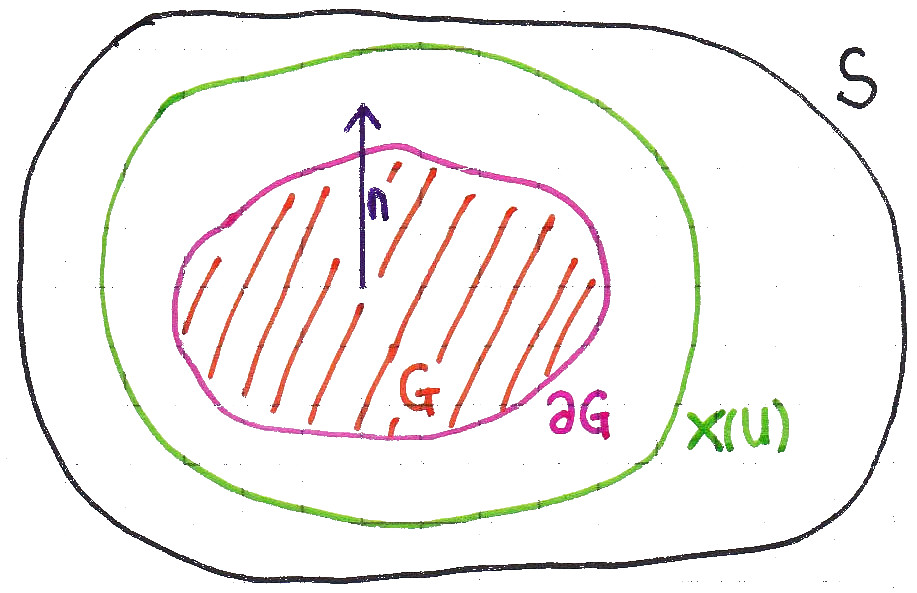
\includegraphics[width=\textwidth]{GaussBonnetLokal}
    \end{figure}
  \end{minipage}
  \begin{proof}
    Definiere ein ``Bezugs-Vektorfeld'' auf \( x(U) \subset S \): \( e \coloneqq \frac{x_u}{\left\Vert x_u \right\Vert} \). Da \( \left\Vert e \right\Vert = 1 \) folgt \( D_u e \perp e \) (La2). Weiter ist nach Definition \( e \perp n \), also \( D_u e \) parallel zu \( n \wedge e \). Also \( D_u e \eqqcolon P(n \wedge e) \) für eine \( C^\infty \)-Funktion \( P : U \to \R \). Analog \( D_v e \eqqcolon Q(n \wedge e) \) für \( C^\infty \)-Funktion \( Q: U \to \R \). \\
    Sei jetzt \( c(s) = x(u(s),v(s)) \) die mit Bogenlänge parametrisierte Kurve, die \( \delta G \) beschreibt. Betrachte \( e \) längs \( c \): \( e(s) \coloneqq e(c(s)) \). Dann

    \begin{minipage}{.6\textwidth}
      \begin{equation*}
        e' = \frac{\text{d}e}{\text{d}s} = e_u u' + e_v v'\text{.}
      \end{equation*}
      Wegen \( e_u = D_u e + \left\langle e_u,n \right\rangle n \) ist
      \begin{align*}
        P &= \left\langle D_u e, n \wedge e \right\rangle = \left\langle e_u, n \wedge e \right\rangle\text{, analog} \\
        Q &= \left\langle e_v, n \wedge e \right\rangle\text{.}
      \end{align*}
    \end{minipage}
    \hfill
    \begin{minipage}{.375\textwidth}
      \begin{figure}[H]
        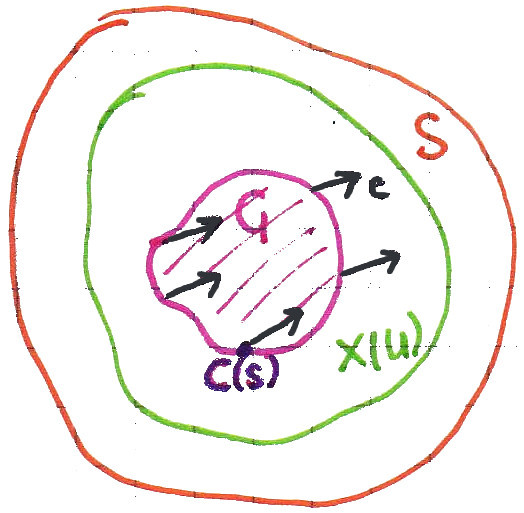
\includegraphics[width=.6\textwidth]{GaussBonnetLokalBeweis}
      \end{figure}
      \vspace*{0.5em}
    \end{minipage}

    Wir betrachten jetzt die linke Seite der Stokesschen Formel. Wir erhalten
    \begin{equation}\label{eq:GB1}
      \int_{\delta G} (Pu' + Qv')\text{d}s = \int_{\delta G}\left\langle \underbrace{e_u u' + e_v v'}_{=e'}, n \wedge e \right\rangle \text{d}s = \int_{\delta G}\left\langle e', n \wedge e \right\rangle \text{d}s\text{.}
    \end{equation}
    Da \( \left\Vert c' \right\Vert = 1 \) können wir schreiben
    \begin{equation}\label{eq:GB2}
      c'(s) = \cos\theta(s)e(s) + \sin\theta(s)(n \wedge e)\text{.}
    \end{equation}
    Weiter ist
    \begin{equation*}
      c''(s) = \frac{\text{d}^2}{\text{d}s^2}c(s) = \kappa_g(n \wedge e') + \alpha n = \alpha n + \kappa_g(\cos\theta(n \wedge e)) + \sin\theta(n \wedge (n \wedge e))e\text{,}
    \end{equation*}
    also
    \begin{equation}\label{eq:GB3}
      \left\langle c'', n \wedge e \right\rangle = \kappa_g\cos\theta\text{.}
    \end{equation}
    Aus \autoref{eq:GB1} ergibt sich:
    \begin{equation*}
      c'' = \cos\theta e' + (\cos\theta)'e + \sin\theta(n \wedge e)' + (\sin\theta)'(n\wedge e)\text{,}
    \end{equation*}
    also
    \begin{equation}\label{eq:GB4}
      \left\langle c'', n \wedge e \right\rangle = \cos\theta \left\langle e', n \wedge e \right\rangle + (\sin\theta)' = \cos\theta\left(\left\langle e', n \wedge e \right\rangle + \theta'\right)\text{.}
    \end{equation}
    Vergleich von 1.3 und 1.4 ergibt \( \kappa_g = \left\langle e', n \wedge e \right\rangle + \theta' \) und somit wegen 1.1:
    \begin{equation*}
      \int_{\delta G}(Pu' + Qv')\text{d}s = \int_{\delta G}\kappa_g\text{d}s - \int_{\delta G}\kappa_g\text{d}s - \theta(s)\vert_{0}^{2\pi} = \int_{\delta G}\kappa_g\text{d}s - 2\pi\text{.}
    \end{equation*}
    Betrachte jetzt die rechte Seite von Lemma 1. Es ist
    \begin{align*}
      D_v D_u e &\underset{\text{Def }P}{=}D_v(P(n \wedge e)) = P_v(n \wedge e) + P(n\wedge e)v - \underbrace{\text{ Normalkomp.\ von } [\cdots]}_{\eqqcolon \beta_n} \\ &\overset{(\star\star)}{=} P_v(n \wedge e) + P(n \wedge e_v)\text{.}
    \end{align*}
    \( (\star\star) \): \( {(n\wedge e)}_v = \underset{\text{normal}}{n_v \wedge e} + \underset{\text{tangential}}{n \wedge e_v} \), also \( {(n \wedge e)}_v = 0 \). \\
    Weiter ist \( n \wedge e_v = n \wedge D_v e \) (da \( D_v e = e_v + \alpha n \) und \( n \wedge n = 0 \)). Also:
    \begin{align*}
      D_v D_u e &= P_v(n \wedge e) + P(n \wedge D_v e) \overset{\text{Def }Q}{=} P_v(n \wedge e) + P(n \wedge Q(n \wedge e)) \\ &= P_v(n \wedge e) + PQ(n \wedge n \wedge e)\text{.}
    \end{align*}
    Vertauschen von \( u,v \) und Subtrahieren ergibt
    \begin{equation*}
      (D_u D_v - D_v D_u)e = (P_v - Q_u)n \wedge e = (K\sqrt{EG - F^2})n \wedge e\text{.}
    \end{equation*}
    Somit
    \begin{align*}
      (P_v - Q_u) &= K\sqrt{EG - F^2} \enskip \text{und} \enskip (P_v - Q_u)\text{d}u\text{d}v &= K\sqrt{EG - F^2}\text{d}u\text{d}v = K\text{d}A\text{.}
    \end{align*}
    Also ist die rechte Seite von Stokes:
    \begin{equation*}
      \iint(Q_u - P_v)\text{d}u\text{d}v = -\iint K\text{d}A\text{.} \hfill \text{\qed}
    \end{equation*}
  \end{proof}
\end{theorem}

\begin{remark}[Bemerkungen zu Gauß-Bonnet]
  \
  \begin{enumerate}
    \item Im Beweis kommt folgender Term vor:
    \begin{equation*}
      \int_{\delta G}\theta' \text{d}s = \theta \vert_0^L = \theta(L) - \theta(0) = 2\pi\text{.}
    \end{equation*}
    \textbf{emph}: \( \theta(s) \) ist eindeutig, falls \( \theta(s) \in [0,2\pi) \). Dann gilt \( \theta(0) = \theta(L) \). \\
    Man benötigt eine Winkelfunktion \( \theta: [0,L] \to \R \) und muss dann zeigen, dass für einfach geschlossene Kurven gilt: \( \theta(L) - \theta(0) = 2\pi \). \\
    Das ist nicht trivial und Inhalt des sogenannten ``Umlaufsatzes von Hopf''.

    \item \emph{Was misst die geodätische Krümmung?} \\
    Sei beispielsweise \( S = \) Ebene. Welche Kurven \( c \in S \) haben \( \kappa_g = 0 \)? Es ist
    \begin{equation*}
      \kappa_g = 0 \Leftrightarrow c'' \Vert n \Leftrightarrow c'' \perp \text{ Tangentialebene } T_{c(s)}S\text{.}
    \end{equation*}
    Für eine Kurve in \( S = \) Ebene ist \( c' \in T_{c(s)}S = T_{c(s)}E = E \). Ebenso ist \( c'' \in E \).
    \begin{align*}
      \text{Also } c'' \perp E &\Leftrightarrow c'' = 0 \\
       &\underset{\mathclap{\text{2-mal integrieren}}}{\Leftrightarrow} c = \text{ parametrisierte Gerade.}
    \end{align*}
  \end{enumerate}  
\end{remark}

\begin{definition}[Geodätische]
  Eine Flächenkurve mit \( \kappa_g = 0 \) heißt \term{Geodätische}\label{def:geodaetische} (Analogon zu Geraden auf krummen Flächen). Man kann zeigen: Geodätische sind lokal kürzeste Verbindungen.
\end{definition}

\begin{example}[Geodätische]
  \
  \begin{enumerate}
    \item \emph{Kugel}: \( S = S_R^2 \). Mit Bogenlänge parametrisierte Großkreise sind Geodätische (haben also \( \kappa_g = 0 \)). \\
      Denn: \( c'' \Vert n \). \( \left\Vert c' \right\Vert^2 = 1 \Leftrightarrow \left\langle c', c' \right\rangle = 1 \underset{\mathclap{\text{ableiten}}}{\Rightarrow} 2\left\langle c', c'' \right\rangle = 0 \).
    
    \item \emph{Zylinder}: \( x(u,v) = \left( \cos u, \sin u, v \right) \). \\
      \( c(s) = \left( \cos(as),\sin(as),bs \right) \), also Bilder unter \( x \) von \( \left( u(s), v(s) \right) = (as, bs) \) (\( = \) Gerade im Parametergebiet \( U \)). Also
      \begin{equation*}
        c'(s) = \left( -a\sin (as), a\cos(as), b \right)\text{.}
      \end{equation*}
      \( s = \) Bogenlänge \( \Leftrightarrow \left\Vert c'(s) \right\Vert = 1 \Leftrightarrow a^2+b^2= 1 \). Es ist
      \begin{equation*}
        c''(s) = \left( -a^2\cos(as), -a^2\sin(as),0 \right)\text{,}
      \end{equation*}
      also \( c'' \Vert n \), also ist \( c(s) \) Geodätische. Es ist:
      \begin{align*}
        a = 0, \ b = 1 &\Rightarrow \text{ Mantellinie} \\
        a = 1, \ b = 0 &\Rightarrow \text{ Breitenkreis} \\
        \text{sonst } &\Rightarrow \text{ Schraubenkurve}
      \end{align*}
  \end{enumerate}
\end{example}

\section{Gauß-Bonnet --- Zweite lokale Version für ``Gebiete mit Ecken''}

Sei \( G \) ein Gebiet mit nur stückweise glattem Rand, \( m \) Ecken bei \( c(t_i) \) (\( i = 1,\dots,m \)). Es sei \( c'(t_i^+) \) die rechtsseitige und \( c'(t_i^-) \) die linksseitige Ableitung bei \( t_i \). Es sei \( \delta_i \) der Außenwinkel zwischen den beiden Tangenten an \( c(t_i) \).

\begin{figure}[H]
  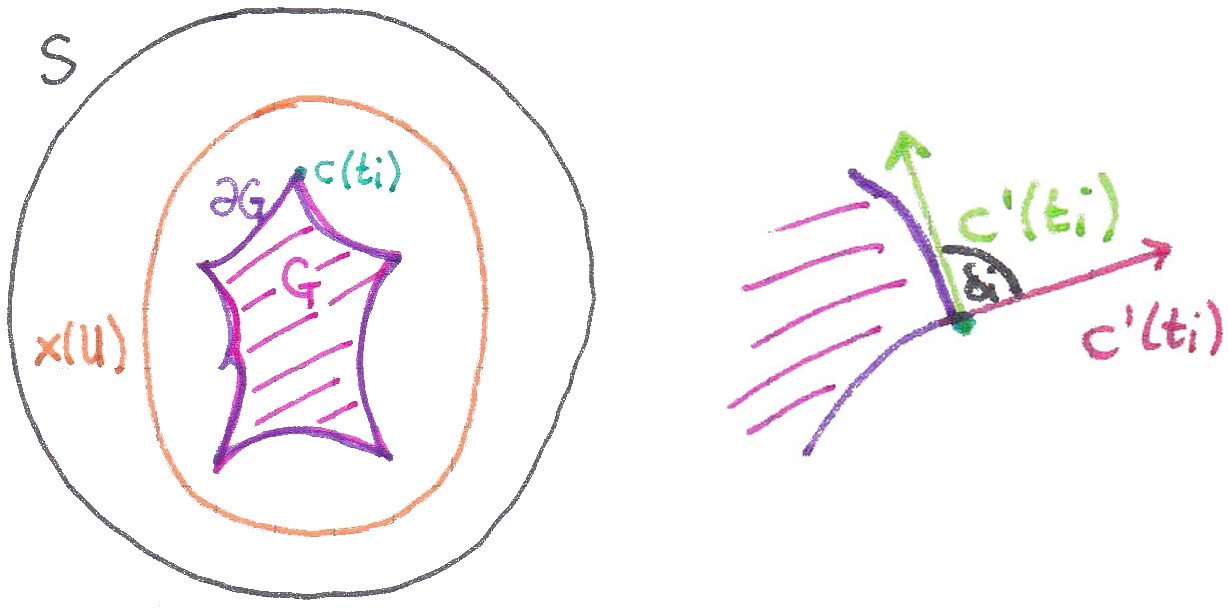
\includegraphics[width=.8\textwidth]{GaussBonnetLokalEcken}
\end{figure}

Sowohl Satz als auch Beweis der zweiten lokalen Version ähneln der ersten --- anstelle des Terms
\begin{equation*}
  \int_{\delta G}\theta'\text{d}s = 2\pi \quad \text{kommt} \quad  \int_{\delta G}\theta'\text{d}s + \sum_{i = 1}^n\delta_i = 2\pi \quad \text{(Umlaufsatz).}
\end{equation*}
Mit \( \alpha_i \coloneqq \pi - \delta_i \) (\emph{Innenwinkel}) für \( i = 1,\dots,m \) ergibt sich
\begin{equation*}
  \iint_G K\text{d}A + \iint_{\delta G}\kappa_g\text{d}s = \pi(2-m) + \sum_{i = 1}^m\alpha_i\text{.}
\end{equation*}


\begin{minipage}{.675\textwidth}
  \begin{remark}[Spezialfall]
    Gauß-Bonnet für geodätische Dreiecke mit Innenwinkel \( \alpha,\beta,\gamma \) (also \( G = \) Dreieck mit geodätischen Segmenten als Randkurven):
    \begin{equation*}
      \iint_\triangle K\text{d}A = \alpha + \beta + \gamma -\pi\text{.}
    \end{equation*}
  \end{remark}  
\end{minipage}
\hfill
\begin{minipage}{.3\textwidth}
  \begin{figure}[H]
    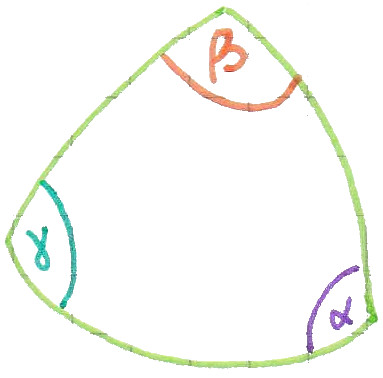
\includegraphics[width=.8\textwidth]{FettesDreieck}
  \end{figure}
\end{minipage}

\begin{remark}[Spezialfälle des Spezialfalls]
  \
  \begin{enumerate}

    \item \( S = \) Ebene, also \( K \equiv 0 \leadsto \) Gauß-Bonnet in Ebene:
    \begin{equation*}
      \alpha + \beta + \gamma = \pi\text{.}
    \end{equation*}

    \begin{minipage}{.675\textwidth}
      \item \( S = S_1^2 =  \) Einheitssphäre hat \( K \equiv 1 \). Sei \( \triangle = \) geodätisches Dreieck auf \( S \):
      \begin{equation*}
        \underbrace{\iint_\triangle 1\text{d}A}_{\text{Flächeninhalt } \triangle} + 0 = \alpha + \beta + \gamma - \pi
      \end{equation*}
      Der Flächeninhalt des (nicht-entarteten) Dreiecks ist \( > 0 \), also \( \alpha + \beta + \gamma > \pi \). Deswegen sehen Dreiecke auf der Einheitssphäre so fett aus.

      \item Flächen mit \( K \equiv -1 \), z.B. Rotationsfläche einer Traktix (Schleppkurve):
      \begin{equation*}
        \underbrace{\iint_\triangle -1\text{d}A}_{< 0} + 0 = \alpha + \beta + \gamma - \pi
      \end{equation*}
      Das Integral ist \( < 0 \), also \( \alpha + \beta + \gamma < \pi \). Deswegen sehen Dreiecke auf solchen Flächen so dünn aus.
    \end{minipage}
    \hfill
    \begin{minipage}{.3\textwidth}
      \begin{figure}[H]
        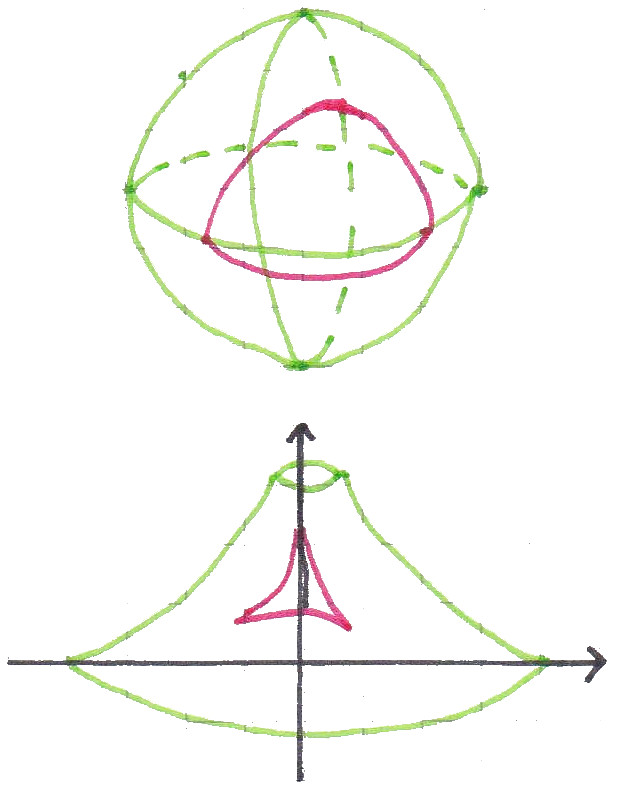
\includegraphics[width=\textwidth]{Traktix}
      \end{figure}
    \end{minipage}

  \end{enumerate}
\end{remark}

\section{Satz von Gauß-Bonnet --- globale Version}

\begin{theorem}[Klassifikationssatz für 2-Mannigfaltigkeiten]
  Eine kompakte randlose \( 2 \)-Mannigfaltigkeit ist entweder zu einer Sphäre \( S^2 \), zu einer zusammenhängenden Summe von \( g \) Tori (falls \( M \) orientierbar ist) oder zu einer zusammenhängenden Summe von \( g \) projektiven Ebenen (falls \( M \) nicht orientierbar ist) homöomorph. \\
  Weiter sind kompakte orientierbare \( 2 \)-Mannigfaltigkeiten mit gleichem \( g \) homöomorph. \( g \) ist also eine topologische Invariante, das sog. \term{Geschlecht}\label{def:geschlecht} der \( 2 \)-Mannigfaltigkeit.
  \begin{proof}
    ohne Beweis. Siehe z.B. Messey, Algebraic Topology. \qed{}
  \end{proof}
\end{theorem}

\begin{figure}[H]
  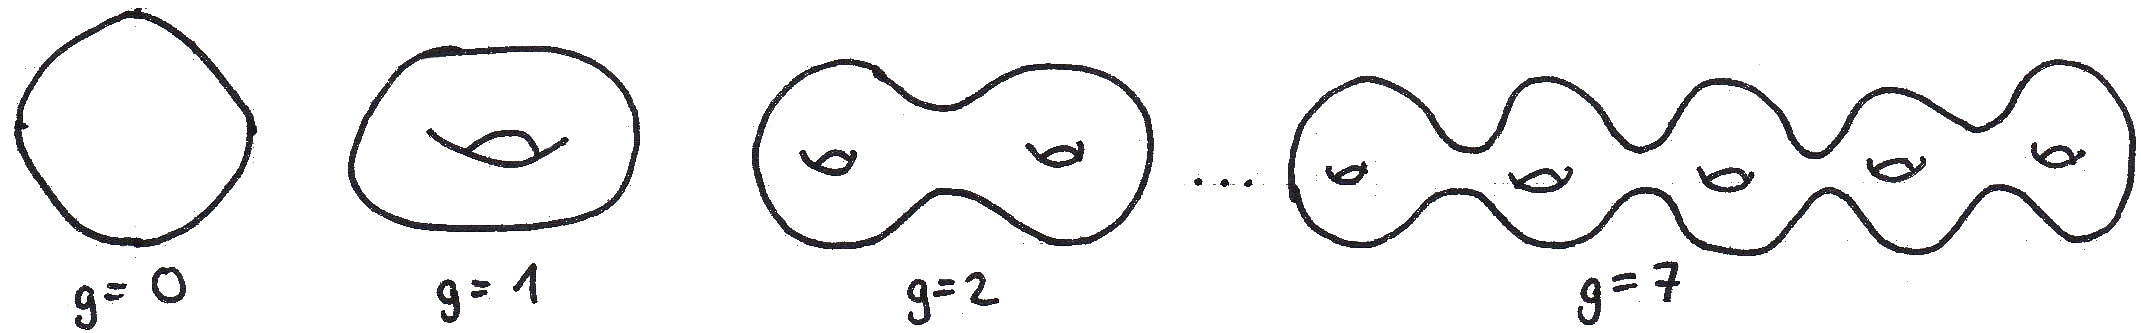
\includegraphics[width=.8\textwidth]{Liste2Mannigfaltigkeiten}
  \caption{Liste der orientierbaren, kompakten \( 2 \)-Mannigfaltigkeiten}
\end{figure}

\begin{definition}[Triangulierung --- Approximation durch Simplizialkomplexe]
  Es sei \( M \) eine kompakte, orientierbare \( 2 \)-Mannigfaltigkeit. Eine \term{Triangulierung}\label{def:triangulierung} von \( M \) ist eine endliche Familie
  \begin{equation*}
    \sigma_k : \underset{\mathclap{\substack{\text{Standard} \\ 2\text{-Simplex}}}}{\triangle} \mapsto \sigma_k(\triangle) \subset M \quad k = 1,\dots,m
  \end{equation*}
  von (orientierungserhaltenden) Diffeomorphismen, für die gilt:
  \begin{enumerate}
    \item Die Simplices \( \sigma_k(\triangle) \) bilden eine Überdeckung von \( M \):
    \begin{equation*}
      M = \bigcup_{k = 1}^m \sigma_k(\triangle)
    \end{equation*}

    \begin{minipage}{.45\textwidth}
      \item Ist \( \sigma_k(\triangle) \cap \sigma_j(\triangle) \neq \varnothing \) (\( k \neq j \)), so haben \( \sigma_k(\triangle) \) und \( \sigma_j(\triangle) \) entweder genau eine Kante oder genau eine Ecke gemeinsam.
    \end{minipage}
    \hfill
    \begin{minipage}{.525\textwidth}
      \begin{figure}[H]
        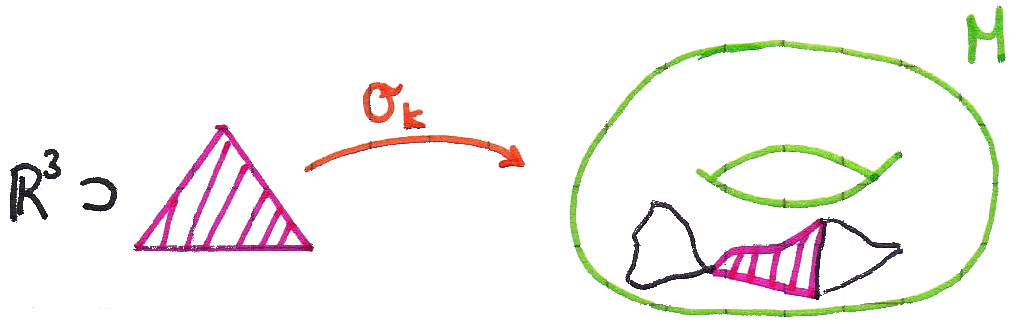
\includegraphics[width=.8\textwidth]{Triangulierung}
      \end{figure}
    \end{minipage}
  \end{enumerate}
  \  \\

  Die \term{Euler-Charakteristik} einer Triangulierung \( T \) von \( M \) ist definiert als
  \begin{equation*}
    \chi_T(M) \coloneqq \#\text{Ecken} - \#\text{Kanten} + \#\text{Flächen.}
  \end{equation*}
\end{definition}

\begin{theorem}[Euler-Charakteristik und Geschlecht]
  \
  \begin{enumerate}
    \item \( \chi(M) \coloneqq \chi_T(M) \) ist unabhängig von der Wahl der Triangulierung.
    \item Es gilt
    \begin{equation*}
      \chi_T(M) = 2-2g \quad (g = \text{ Geschlecht von } M)
    \end{equation*}
  \end{enumerate}
  Insbesondere gilt nach dem Klassifikationssatz, dass \( \chi(M) \) eine topologische Invariante ist.
  \begin{proof}
    Beweisskizze.
    \begin{enumerate}
      \item Folgt aus dem Satz von Gauß-Bonnet, mehr dazu später. \qed{}
      \item Es ist \( \chi(T^2) = 0 \). Nehmen wir ein Dreieck heraus, so ist \( \chi(T^2 \setminus \dot{\triangle}) = \chi(T^2) - 1 = -1 \). Es ist also
      \begin{equation*}
        \chi(T^2 \# T^2) = -2 = 2 - 2*2\text{.}
      \end{equation*}
      Mit Induktion:
      \begin{equation*}
        \chi(\underbrace{T^2 \# \cdots \# T^2}_{k \text{ Summanden}}) = 2-2g\text{.}
      \end{equation*}
      \qed{}
    \end{enumerate}
  \end{proof}
\end{theorem}

\begin{theorem}[Beinhalten von Triangulierungen]
  Jede kompakte, orientierbare \( 2 \)-Mannigfaltigkeit mit gegebenem Atlas \( \mathcal{A} \) besitzt eine Triangulierung
  \begin{equation*}
    \sigma_k : \delta \to M\text{,} \quad k = 1,\dots,m\text{,}
  \end{equation*}
  sodass jedes Simplex \( \sigma_k(\triangle) \) ganz im Definitionsbereich einer Karte (also dem Bild einer Parametrisierung) von \( \mathcal{A} \) enthalten ist. \\
  Dieser Satz erlaubt den Übergang vom lokalen Gauß-Bonnet-Satz zum globalen.
\end{theorem}

\begin{theorem}[Globaler Satz von Gauß-Bonnet]
  Es sei \( S \subset \R^3 \) eine kompakte randlose orientierbare Fläche. Dann gilt:
  \begin{equation*}
    \overbrace{\iint_S K\text{d}A}^{\mathclap{\text{geometrische Größe}}} = \underbrace{2\pi\chi(S)}_{\mathclap{=2\pi(2-2g)\text{, topologische Größe}}}\text{.}
  \end{equation*}
  \begin{proof}
    Wähle eine Triangulierung \( \sigma_j: \triangle \to S \) (\( j = 1,\dots,f \)) sodass alle Dreiecke \( \sigma_j(\triangle) \) ganz in einem Kartengebiet \( x_j(U_j) \) liegen. Wie orientieren die Ränder der Dreiecke, sodass sie mit der Orientierung von \( S \) übereinstimmen. \\
    Sei \( e \coloneqq \# \) Ecken, \( k \coloneqq \# \) Kanten, \( f \coloneqq \# \) Flächen. \\
    Aus der lokalen Version des Satzes von Gauß-Bonnet folgt, dass für jedes Dreieck gilt:
    \begin{equation*}
      \iint_{\sigma_j(\triangle)}K\text{d}A = -\int_{\delta(\sigma_j(\triangle))}\kappa_g\text{d}s + \sum_{i = 1}^3 \alpha_i^{(j)} - \pi
    \end{equation*}
    Summieren über \( j = 1,\dots,f \) ergibt:
    \begin{equation*}
      \iint_S K\text{d}A = \sum_{j=1}^f\iint_{\sigma_j(\triangle)}K\text{d}A = -\sum_{j=1}^f\int_{\delta(\sigma_j(\triangle))}\kappa_g\text{d}s + e*2\pi + f*\pi \text{.}
    \end{equation*}
    Jede Dreieckskante erscheint in dieser Summe \( 2 \) mal, aber gegenläufig orientiert. Da die geodätische Krümmung das Vorzeichen ändert, wenn die Kurven/Kanten gegenläufig durchlaufen werden, hebt sich der \( \kappa_g \)-Term auf --- also:
    \begin{equation*}
      \iint_S K\text{d}A = e*2\pi + f*\pi
    \end{equation*}
    Jede Dreiecksfläche hat \( 3 \) Kanten, jede Kante berandet \( 2 \) Dreiecksflächen, also \( 3f = 2k \) und somit
    \begin{equation*}
      \iint_S K\text{d}A = 2\pi e - f\pi = 2\pi(e - \frac{3}{2}f + f) = 2\pi(e-k+f) = 2\pi\chi(S)\text{.}
    \end{equation*} \qed{}
  \end{proof}
\end{theorem}

\begin{remark}
  Der Satz gilt allgemein für kompakte orientierbare \( 2 \)-Mannigfaltigkeiten, die nicht unbedingt in den \( \R^3 \) eingebettet sein müssen. Dazu muss man die Begriffe wie Tangentialebene, erste Fundamentalform, Krümmung usw.\ verallgemeinern (siehe Vorlesung Differentialgeometrie). \\
  Die Topologie schränkt die Möglichkeiten für die Geometrie ein (und umgekehrt) --- beispielsweise gilt, dass die meisten Flächen negative Euler-Charakteristik haben. Also kann die Krümmung nicht überall \( \geq 0 \) sein. Ist beispielsweise \( K \equiv 0 \), so muss \( \chi(S) = 0 \Leftrightarrow g = 1 \) gelten.
\end{remark}

\begin{minipage}{.45\textwidth}
  \begin{figure}[H]
    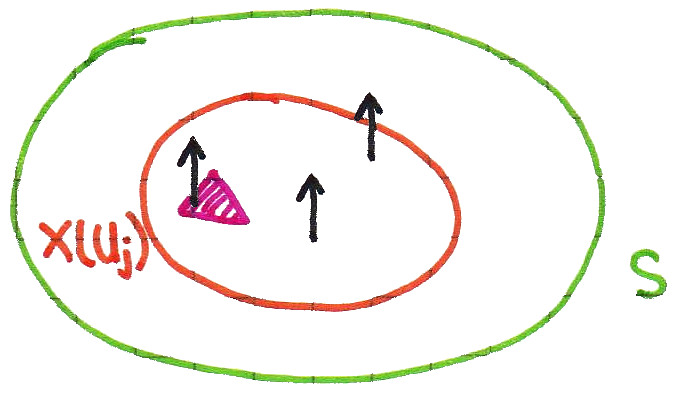
\includegraphics[width=.8\textwidth]{GaussBonnetLokalVergleich}
    \vspace*{1em}
    \caption{Lokaler Satz von Gauß-Bonnet}
  \end{figure}
\end{minipage}
\hfill
\begin{minipage}{.475\textwidth}
  \begin{figure}[H]
    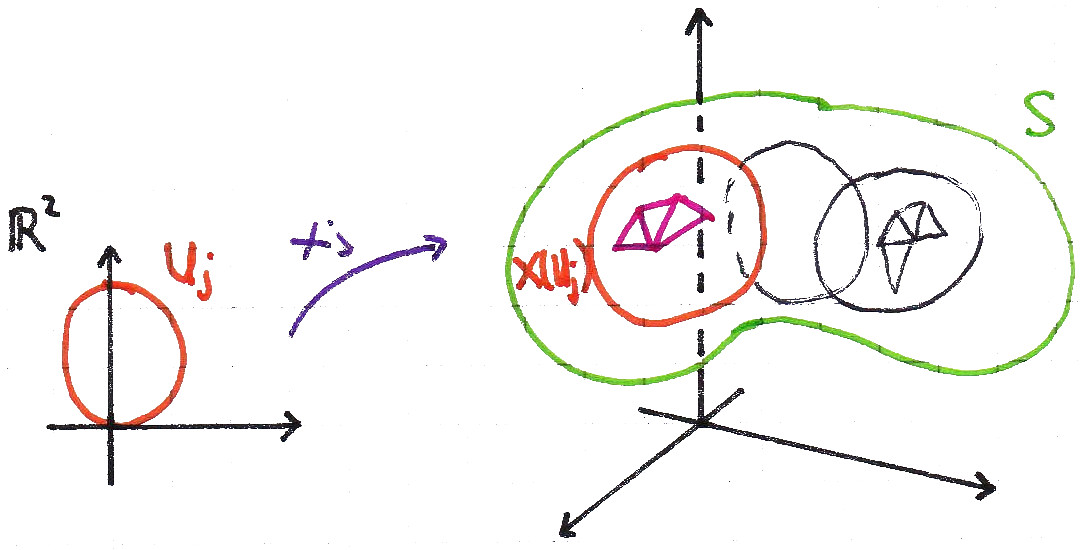
\includegraphics[width=\textwidth]{GaussBonnetGlobalVergleich}
    \caption{Globaler Satz von Gauß-Bonnet}
  \end{figure}
\end{minipage}
